\PassOptionsToPackage{table}{xcolor}
\documentclass{beamer}

% xcolor and define colors -------------------------
\usepackage[table]{xcolor}

% https://www.viget.com/articles/color-contrast/
\definecolor{purple}{HTML}{5601A4}
\definecolor{navy}{HTML}{0D3D56}
\definecolor{ruby}{HTML}{9a2515}
\definecolor{alice}{HTML}{107895}
\definecolor{daisy}{HTML}{EBC944}
\definecolor{coral}{HTML}{F26D21}
\definecolor{kelly}{HTML}{829356}
\definecolor{cranberry}{HTML}{E64173}
\definecolor{jet}{HTML}{131516}
\definecolor{asher}{HTML}{555F61}
\definecolor{slate}{HTML}{314F4F}

% Mixtape Sessions
\definecolor{picton-blue}{HTML}{00b7ff}
\definecolor{violet-red}{HTML}{ff3881}
\definecolor{sun}{HTML}{ffaf18}
\definecolor{electric-violet}{HTML}{871EFF}

% Main theme colors
\definecolor{accent}{HTML}{00b7ff}
\definecolor{accent2}{HTML}{871EFF}
\definecolor{gray100}{HTML}{f3f4f6}
\definecolor{gray800}{HTML}{1F292D}

\definecolor{bgRaspberry}{HTML}{ff96a9}
\definecolor{bgCranberry}{HTML}{fda4d0}
\definecolor{bgOrange}{HTML}{f6b97b}
\definecolor{bgPurple}{HTML}{adb4f4}
\definecolor{bgBlue}{HTML}{cdfbff}
\definecolor{bgGreen}{HTML}{8ee7af}
\definecolor{bgRose}{HTML}{fecdd4}
\definecolor{bgYellow}{HTML}{ffea88}

% Beamer Options -------------------------------------

% Background
\setbeamercolor{background canvas}{bg = white}

% Change text margins
\setbeamersize{text margin left = 15pt, text margin right = 15pt}

% \alert
\setbeamercolor{alerted text}{fg = accent2}

% Frame title
\setbeamercolor{frametitle}{bg = white, fg = jet}
\setbeamercolor{framesubtitle}{bg = white, fg = accent}
\setbeamerfont{framesubtitle}{size = \small, shape = \itshape}

% Block
\setbeamercolor{block title}{fg = white, bg = accent2}
\setbeamercolor{block body}{fg = gray800, bg = gray100}

% Title page
\setbeamercolor{title}{fg = gray800}
\setbeamercolor{subtitle}{fg = accent}

%% Custom \maketitle and \titlepage
\setbeamertemplate{title page}
{
    %\begin{centering}
        \vspace{20mm}
        {\Large \usebeamerfont{title}\usebeamercolor[fg]{title}\inserttitle}\\
        {\large \itshape \usebeamerfont{subtitle}\usebeamercolor[fg]{subtitle}\insertsubtitle}\\ \vspace{10mm}
        {\insertauthor}\\
        {\color{asher}\small{\insertdate}}\\
    %\end{centering}
}

% Table of Contents
\setbeamercolor{section in toc}{fg = accent!70!jet}
\setbeamercolor{subsection in toc}{fg = jet}

% Button
\setbeamercolor{button}{bg = accent}

% Remove navigation symbols
\setbeamertemplate{navigation symbols}{}

% Table and Figure captions
\setbeamercolor{caption}{fg=jet!70!white}
\setbeamercolor{caption name}{fg=jet}
\setbeamerfont{caption name}{shape = \itshape}

% Bullet points

%% Fix left-margins
\settowidth{\leftmargini}{\usebeamertemplate{itemize item}}
\addtolength{\leftmargini}{\labelsep}

%% enumerate item color
\setbeamercolor{enumerate item}{fg = accent}
\setbeamerfont{enumerate item}{size = \small}
\setbeamertemplate{enumerate item}{\insertenumlabel.}

%% itemize
\setbeamercolor{itemize item}{fg = accent!70!white}
\setbeamerfont{itemize item}{size = \small}
\setbeamertemplate{itemize item}[circle]

%% right arrow for subitems
\setbeamercolor{itemize subitem}{fg = accent!60!white}
\setbeamerfont{itemize subitem}{size = \small}
\setbeamertemplate{itemize subitem}{$\rightarrow$}

\setbeamertemplate{itemize subsubitem}[square]
\setbeamercolor{itemize subsubitem}{fg = jet}
\setbeamerfont{itemize subsubitem}{size = \small}


% Special characters

\usepackage{collectbox}

\makeatletter
\newcommand{\mybox}{%
    \collectbox{%
        \setlength{\fboxsep}{1pt}%
        \fbox{\BOXCONTENT}%
    }%
}
\makeatother





% Links ----------------------------------------------

\usepackage{hyperref}
\hypersetup{
  colorlinks = true,
  linkcolor = accent2,
  filecolor = accent2,
  urlcolor = accent2,
  citecolor = accent2,
}


% Line spacing --------------------------------------
\usepackage{setspace}
\setstretch{1.1}


% \begin{columns} -----------------------------------
\usepackage{multicol}


% Fonts ---------------------------------------------
% Beamer Option to use custom fonts
\usefonttheme{professionalfonts}

% \usepackage[utopia, smallerops, varg]{newtxmath}
% \usepackage{utopia}
\usepackage[sfdefault,light]{roboto}

% Small adjustments to text kerning
\usepackage{microtype}



% Remove annoying over-full box warnings -----------
\vfuzz2pt
\hfuzz2pt


% Table of Contents with Sections
\setbeamerfont{myTOC}{series=\bfseries, size=\Large}
\AtBeginSection[]{
        \frame{
            \frametitle{Roadmap}
            \tableofcontents[current]
        }
    }


% Tables -------------------------------------------
% Tables too big
% \begin{adjustbox}{width = 1.2\textwidth, center}
\usepackage{adjustbox}
\usepackage{array}
\usepackage{threeparttable, booktabs, adjustbox}

% Fix \input with tables
% \input fails when \\ is at end of external .tex file
\makeatletter
\let\input\@@input
\makeatother

% Tables too narrow
% \begin{tabularx}{\linewidth}{cols}
% col-types: X - center, L - left, R -right
% Relative scale: >{\hsize=.8\hsize}X/L/R
\usepackage{tabularx}
\newcolumntype{L}{>{\raggedright\arraybackslash}X}
\newcolumntype{R}{>{\raggedleft\arraybackslash}X}
\newcolumntype{C}{>{\centering\arraybackslash}X}

% Figures

% \imageframe{img_name} -----------------------------
% from https://github.com/mattjetwell/cousteau
\newcommand{\imageframe}[1]{%
    \begin{frame}[plain]
        \begin{tikzpicture}[remember picture, overlay]
            \node[at = (current page.center), xshift = 0cm] (cover) {%
                \includegraphics[keepaspectratio, width=\paperwidth, height=\paperheight]{#1}
            };
        \end{tikzpicture}
    \end{frame}%
}

% subfigures
\usepackage{subfigure}


% Highlight slide -----------------------------------
% \begin{transitionframe} Text \end{transitionframe}
% from paulgp's beamer tips
\newenvironment{transitionframe}{
    \setbeamercolor{background canvas}{bg=accent!40!black}
    \begin{frame}\color{accent!10!white}\LARGE\centering
}{
    \end{frame}
}


% Table Highlighting --------------------------------
% Create top-left and bottom-right markets in tabular cells with a unique matching id and these commands will outline those cells
\usepackage[beamer,customcolors]{hf-tikz}
\usetikzlibrary{calc, fit, shadows, arrows, arrows.meta, shapes.misc, shapes,decorations, decorations.pathreplacing, positioning}
\usepackage[most,skins]{tcolorbox}
\tcbuselibrary{breakable}
\tcbset{
  highlight math/.style={
    notitle, enhanced,
    on line, boxsep=2pt, left=0pt, right=0pt, top=0pt, bottom=0pt,
    colback = bgRaspberry, colframe = white,
  }
}

% To set the hypothesis highlighting boxes red.
\newcommand\marktopleft[1]{%
    \tikz[overlay,remember picture]
        \node (marker-#1-a) at (0,1.5ex) {};%
}
\newcommand\markbottomright[1]{%
    \tikz[overlay,remember picture]
        \node (marker-#1-b) at (0,0) {};%
    \tikz[accent!80!jet, ultra thick, overlay, remember picture, inner sep=4pt]
        \node[draw, rectangle, fit=(marker-#1-a.center) (marker-#1-b.center)] {};%
}


% Define custom slide coordinate system ----------------------------------------
% https://tex.stackexchange.com/questions/89588/positioning-relative-to-page-in-tikz
% Defining a new coordinate system for the page:
%
% ┌──────────────────────────────────────────────┐
% │ (0, 0)                                (1, 0) │
% │                                              │
% │                                              │
% │                                              │
% │                                              │
% │                                              │
% │ (0, 1)                                (1, 1) │
% └──────────────────────────────────────────────┘
%
% source: https://tex.stackexchange.com/questions/89588/positioning-relative-to-page-in-tikz
%
\makeatletter
\def\parsecomma#1,#2\endparsecomma{\def\page@x{#1}\def\page@y{#2}}
\tikzdeclarecoordinatesystem{page}{
    \parsecomma#1\endparsecomma
    \pgfpointanchor{current page}{north west}
    % Save the upper left corner
    \pgf@xa=\pgf@x%
    \pgf@ya=\pgf@y%
    % save the lower right corner
    \pgfpointanchor{current page}{south east}
    \pgf@xb=\pgf@x%
    \pgf@yb=\pgf@y%
    % Transform to the correct placement
    \pgfmathparse{(\pgf@xb-\pgf@xa)*\page@x+\pgf@xa}
    \expandafter\pgf@x\expandafter=\pgfmathresult pt
    \pgfmathparse{(\pgf@yb-\pgf@ya)*\page@y+\pgf@ya}
    \expandafter\pgf@y\expandafter=\pgfmathresult pt
}
\makeatother

% To overlay on beamer slides, use the following:
%
% \begin{tikzpicture}[remember picture, overlay]
%   \node[anchor = north west] (anchor_name) at (page cs:0.0, 0.0) {
%     CONTENT HERE
%   };
% \end{tikzpicture}
%
% Note page cs is the coordinate system from above

% To help with placement, I will use `\devgrid` on a slide to figure out the coordinates of `page cs` to the 0.1
\newcommand{\devgrid}{
  \begin{tikzpicture}[remember picture, overlay]
    % vertical lines
    \draw (page cs: 0.1, 0.0) edge[black!20!white, line width = 0.3mm, dotted] (page cs: 0.1, 1.0);
    \draw (page cs: 0.2, 0.0) edge[black!20!white, line width = 0.3mm, dotted] (page cs: 0.2, 1.0);
    \draw (page cs: 0.3, 0.0) edge[black!20!white, line width = 0.3mm, dotted] (page cs: 0.3, 1.0);
    \draw (page cs: 0.4, 0.0) edge[black!20!white, line width = 0.3mm, dotted] (page cs: 0.4, 1.0);
    \draw (page cs: 0.5, 0.0) edge[black!20!white, line width = 0.3mm, dotted] (page cs: 0.5, 1.0);
    \draw (page cs: 0.6, 0.0) edge[black!20!white, line width = 0.3mm, dotted] (page cs: 0.6, 1.0);
    \draw (page cs: 0.7, 0.0) edge[black!20!white, line width = 0.3mm, dotted] (page cs: 0.7, 1.0);
    \draw (page cs: 0.8, 0.0) edge[black!20!white, line width = 0.3mm, dotted] (page cs: 0.8, 1.0);
    \draw (page cs: 0.9, 0.0) edge[black!20!white, line width = 0.3mm, dotted] (page cs: 0.9, 1.0);

    % horizontal lines
    \draw (page cs: 0.0, 0.1) edge[black!20!white, line width = 0.3mm, dotted] (page cs: 1.0, 0.1);
    \draw (page cs: 0.0, 0.2) edge[black!20!white, line width = 0.3mm, dotted] (page cs: 1.0, 0.2);
    \draw (page cs: 0.0, 0.3) edge[black!20!white, line width = 0.3mm, dotted] (page cs: 1.0, 0.3);
    \draw (page cs: 0.0, 0.4) edge[black!20!white, line width = 0.3mm, dotted] (page cs: 1.0, 0.4);
    \draw (page cs: 0.0, 0.5) edge[black!20!white, line width = 0.3mm, dotted] (page cs: 1.0, 0.5);
    \draw (page cs: 0.0, 0.6) edge[black!20!white, line width = 0.3mm, dotted] (page cs: 1.0, 0.6);
    \draw (page cs: 0.0, 0.7) edge[black!20!white, line width = 0.3mm, dotted] (page cs: 1.0, 0.7);
    \draw (page cs: 0.0, 0.8) edge[black!20!white, line width = 0.3mm, dotted] (page cs: 1.0, 0.8);
    \draw (page cs: 0.0, 0.9) edge[black!20!white, line width = 0.3mm, dotted] (page cs: 1.0, 0.9);
  \end{tikzpicture}
}

\usepackage{breqn} % Breaks lines

\usepackage{amsmath}
\usepackage{mathtools}


\usepackage{pdfpages} % \includepdf

\usepackage{listings} % R code
\usepackage{verbatim} % verbatim

% Video stuff
\usepackage{media9}

% packages for bibs and cites
\usepackage{natbib}
\usepackage{har2nat}
\newcommand{\possessivecite}[1]{\citeauthor{#1}'s \citeyearpar{#1}}
\usepackage{breakcites}
\usepackage{alltt}

% Setup math operators
\DeclareMathOperator{\E}{E} \DeclareMathOperator{\tr}{tr} \DeclareMathOperator{\se}{se} \DeclareMathOperator{\I}{I} \DeclareMathOperator{\sign}{sign} \DeclareMathOperator{\supp}{supp} \DeclareMathOperator{\plim}{plim}
\DeclareMathOperator*{\dlim}{\mathnormal{d}\mkern2mu-lim}
\newcommand\independent{\protect\mathpalette{\protect\independenT}{\perp}}
   \def\independenT#1#2{\mathrel{\rlap{$#1#2$}\mkern2mu{#1#2}}}
\newcommand*\colvec[1]{\begin{pmatrix}#1\end{pmatrix}}

\newcommand{\myurlshort}[2]{\href{#1}{\textcolor{gray}{\textsf{#2}}}}


\begin{document}

\begin{frame}[plain]  % Removes header/footer and gives you full vertical control
\vfill
\begin{center}
  
\includegraphics[width=0.85\linewidth]{./lecture_includes/banner_cropped}
\end{center}
\vfill
\end{frame}


% ---- Content ----


\section{Continuous DiD}

\subsection{Dx2 and DxT}

\begin{frame}{Continuous DiD}

\begin{itemize}
\item It is very common for people to estimate difference-in-differences panel models where the treatment, $D$, is multi-valued or continuous, not binary:

$$Y_{it} = \alpha + \delta D_{it}  + \tau_t + \sigma_s + \varepsilon_{it}$$

\item Examples include minimum wage papers, my JHR on abortion clinic closures causing increased travel distance, vaccinations, price elasticity of demand etc.
\item Variation is in ``treatment intensity'' and researchers typically use TWFE for estimation, or perhaps count models like Poisson

\end{itemize}

\end{frame}


\begin{frame}{Praise for OLS and Continuous Treatments}

\begin{quote}
``The two-period regression estimator can be easily modified to allow for continuous, or at least non-binary, treatments.'' (Wooldridge 2005)

\bigskip

``A second advantage of regression DiD is that it facilitates the study of policies other than those that can be described by a dummy.'' (Angrist and Pischke 2008)

\end{quote}

\end{frame}

\clearpage




\begin{frame}{New Continuous DiD}

\begin{enumerate}
\item But new work suggests that the TWFE approach to continuous is problematic in light of unrestricted heterogenous treatment effects (Baker, et al. 2025)
\item What of the 2x2 and 2xT will be relevant for dosage designs (Dx2 and DxT)?
\item What is the target parameter, what new assumptions, what estimation methods, what control group?
\end{enumerate}

\end{frame}



\begin{frame}{Continuous Literature in Causal Inference}

\begin{itemize}
\item Continuous treatments in instrumental variables (Angrist and Imbens 1995; Angrist, Graddy and Imbens 2000)
\item Continuous instruments (Imbens and Angrist 1994; Heckman and Vytacil 2005)
\item But the work on continuous diff-in-diff is newer (de Chaisemartin, et al. 2024; de Chaisemartin, et al. 2025; Callaway, Goodman-Bacon and Sant'Anna 2025)
\item We will primarily focus on Callaway, Goodman-Bacon and Sant'Anna (2025) for the sake of time and focus

\end{itemize}

\end{frame}

\subsection{Target Parameters}


\begin{frame}{Average causal response functions}


Review of old terms, introducing new terms:

\bigskip

\begin{itemize}
\item \textbf{ATT}: Average effect for a binary treatment on a sub-population of treated units after they were treated (i.e., $E[\delta|D=1]$ for binary treatment)
\item \textbf{Dose}: Treatment is not binary but rather multi-valued or continuous.  Represents either ATTs for groups at dosages, or movements along a dosage curve -- not the same thing as it turns out
\end{itemize}

\end{frame}





\begin{frame}{Dosage Parameters give us a multitude of ATTs}

\begin{block}{Average treated on the treated for a given dose}
$ATT(d|d) = E[Y^d_{it} - \textcolor{red}{Y^0_{it}} | D_{it}=d]$
\end{block}

\begin{itemize}
\item This is a restatement of our original ATT, except we are defining the binary treatment, $D$, at a given dosage $d$. 
\item ``What is the average effect of being 100 kilometers from a hospital compared to being 0 kilometers from a hospital?''
	\begin{itemize}
	\item Notice the counterfactual -- "zero dose" (i.e., $\textcolor{red}{Y^0}$)
	\end{itemize}
\item  This is ``the ATT of dose $d=100$ km for the groups that are at $d=100$ km'' which uses as its comparison no dose (as opposed to a marginally smaller dose)
\end{itemize}

\end{frame}



\begin{frame}{Earlier dosage parameters in causal inference}

\begin{quote}
``We refer to the parameter $\beta$ as the \textbf{average causal response (ACR)}. This parameter captures a weighed average causal responses to a unit change in treatment, for those whose treatment status is affected by the instrument. \dots '' (Angrist and Imbens 1995)
\end{quote}

\end{frame}


\begin{frame}{ATT for a given dose}

\begin{figure}
\begin{center}
             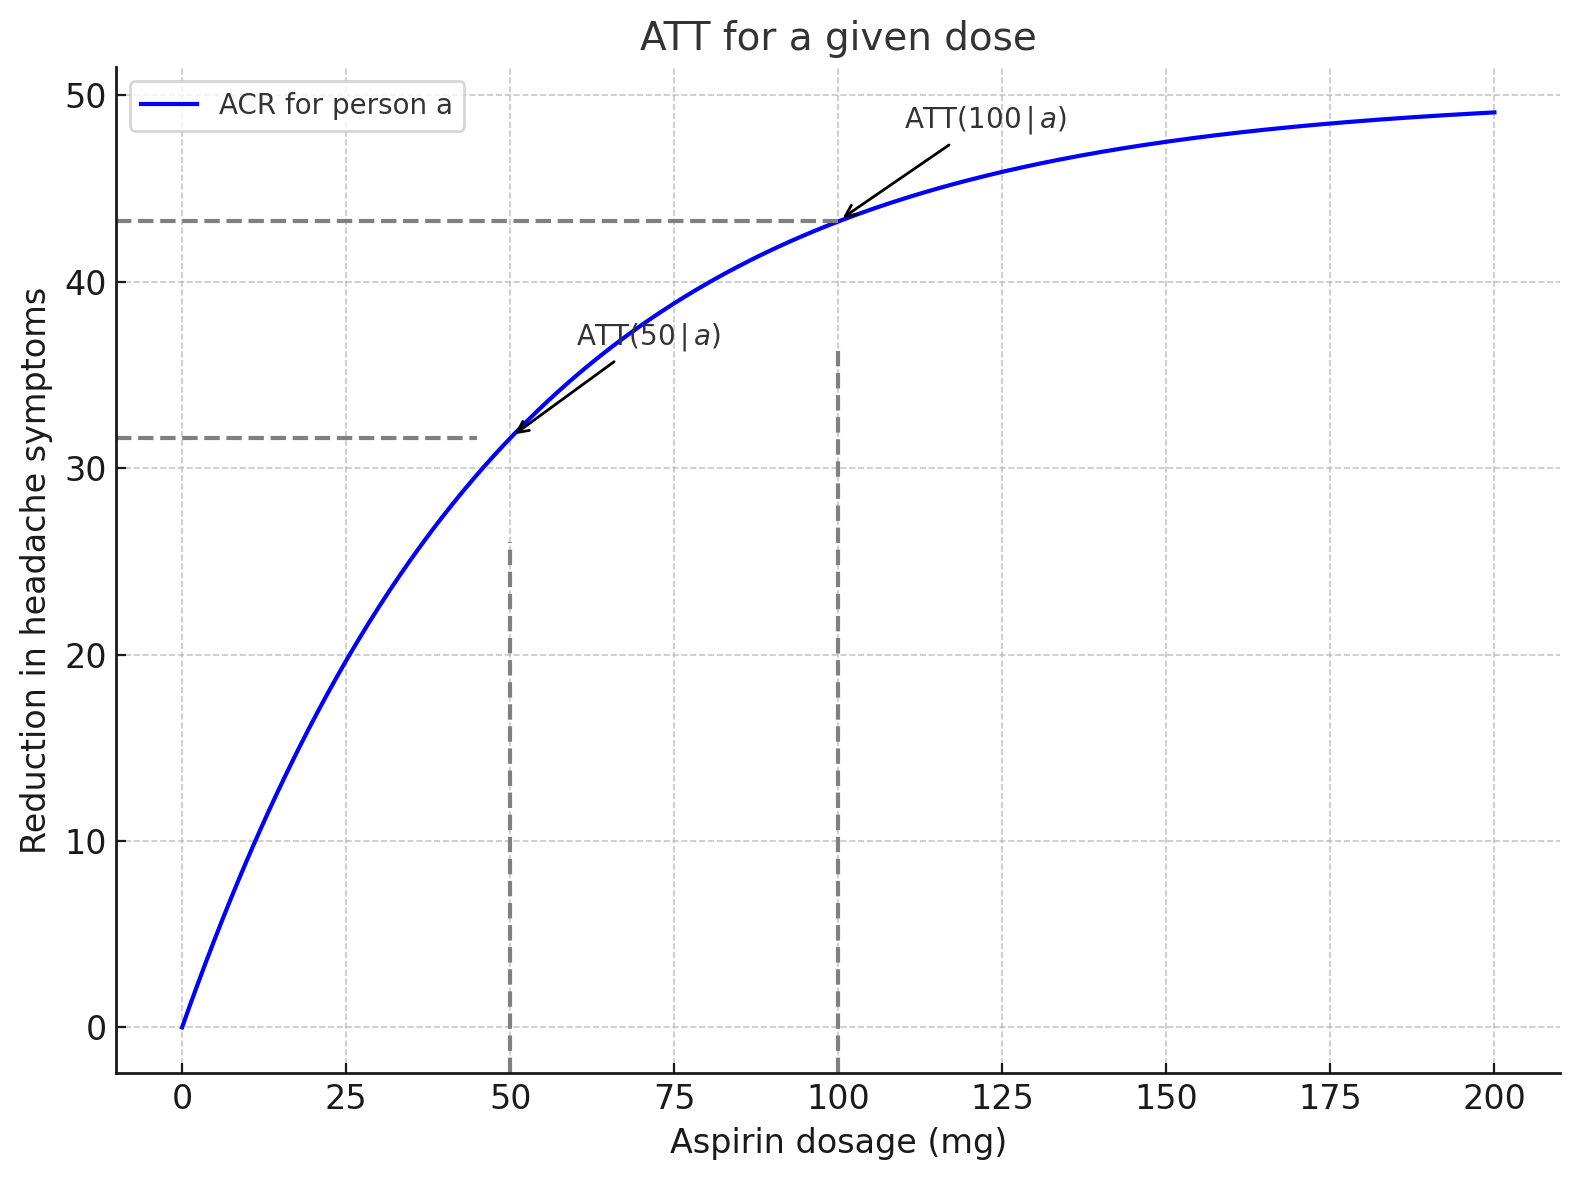
\includegraphics[scale=0.3]{./lecture_includes/acrt_fig1.png}
\end{center}
\end{figure}

What is the effect of aspirin on headache symptoms for a single person?  At 50 mg, the ATT is 31, but at 100mg, it's 44.   


\end{frame}

\begin{frame}{ATT for a given dose}

\begin{figure}
\begin{center}
             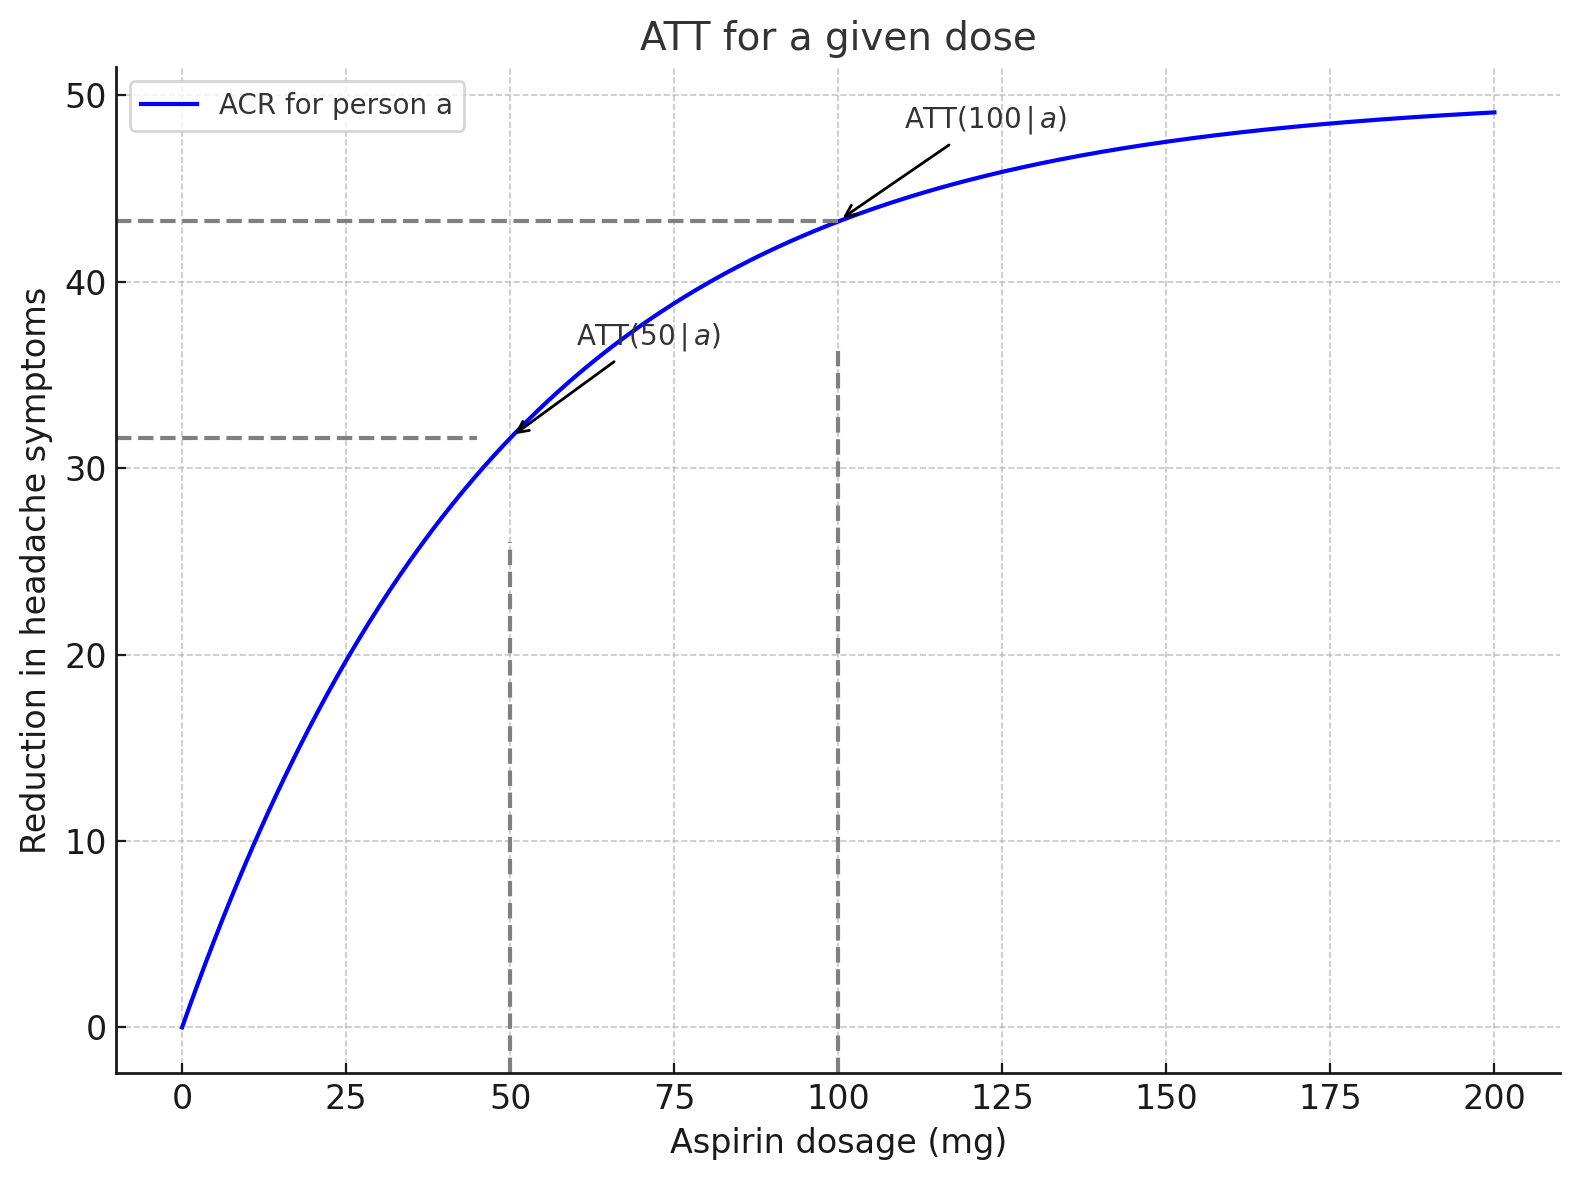
\includegraphics[scale=0.3]{./lecture_includes/acrt_fig1.png}
\end{center}
\end{figure}

\begin{itemize}
\item Assume Giovanni is person $a$ and he chose in reality $d=50$ mg of aspiring.  
\item Then $ATT(100|a)$ is a counterfactual ATT because while it is the same person, it is a dosage that he has not yet taken.  
\item All ATTs have counterfactuals, but the curve maps out not just counterfactual causal effects, but also \emph{counterfactual dosages}
\end{itemize}


\end{frame}


\begin{frame}{ATT for a given dose}

\begin{figure}
\begin{center}
             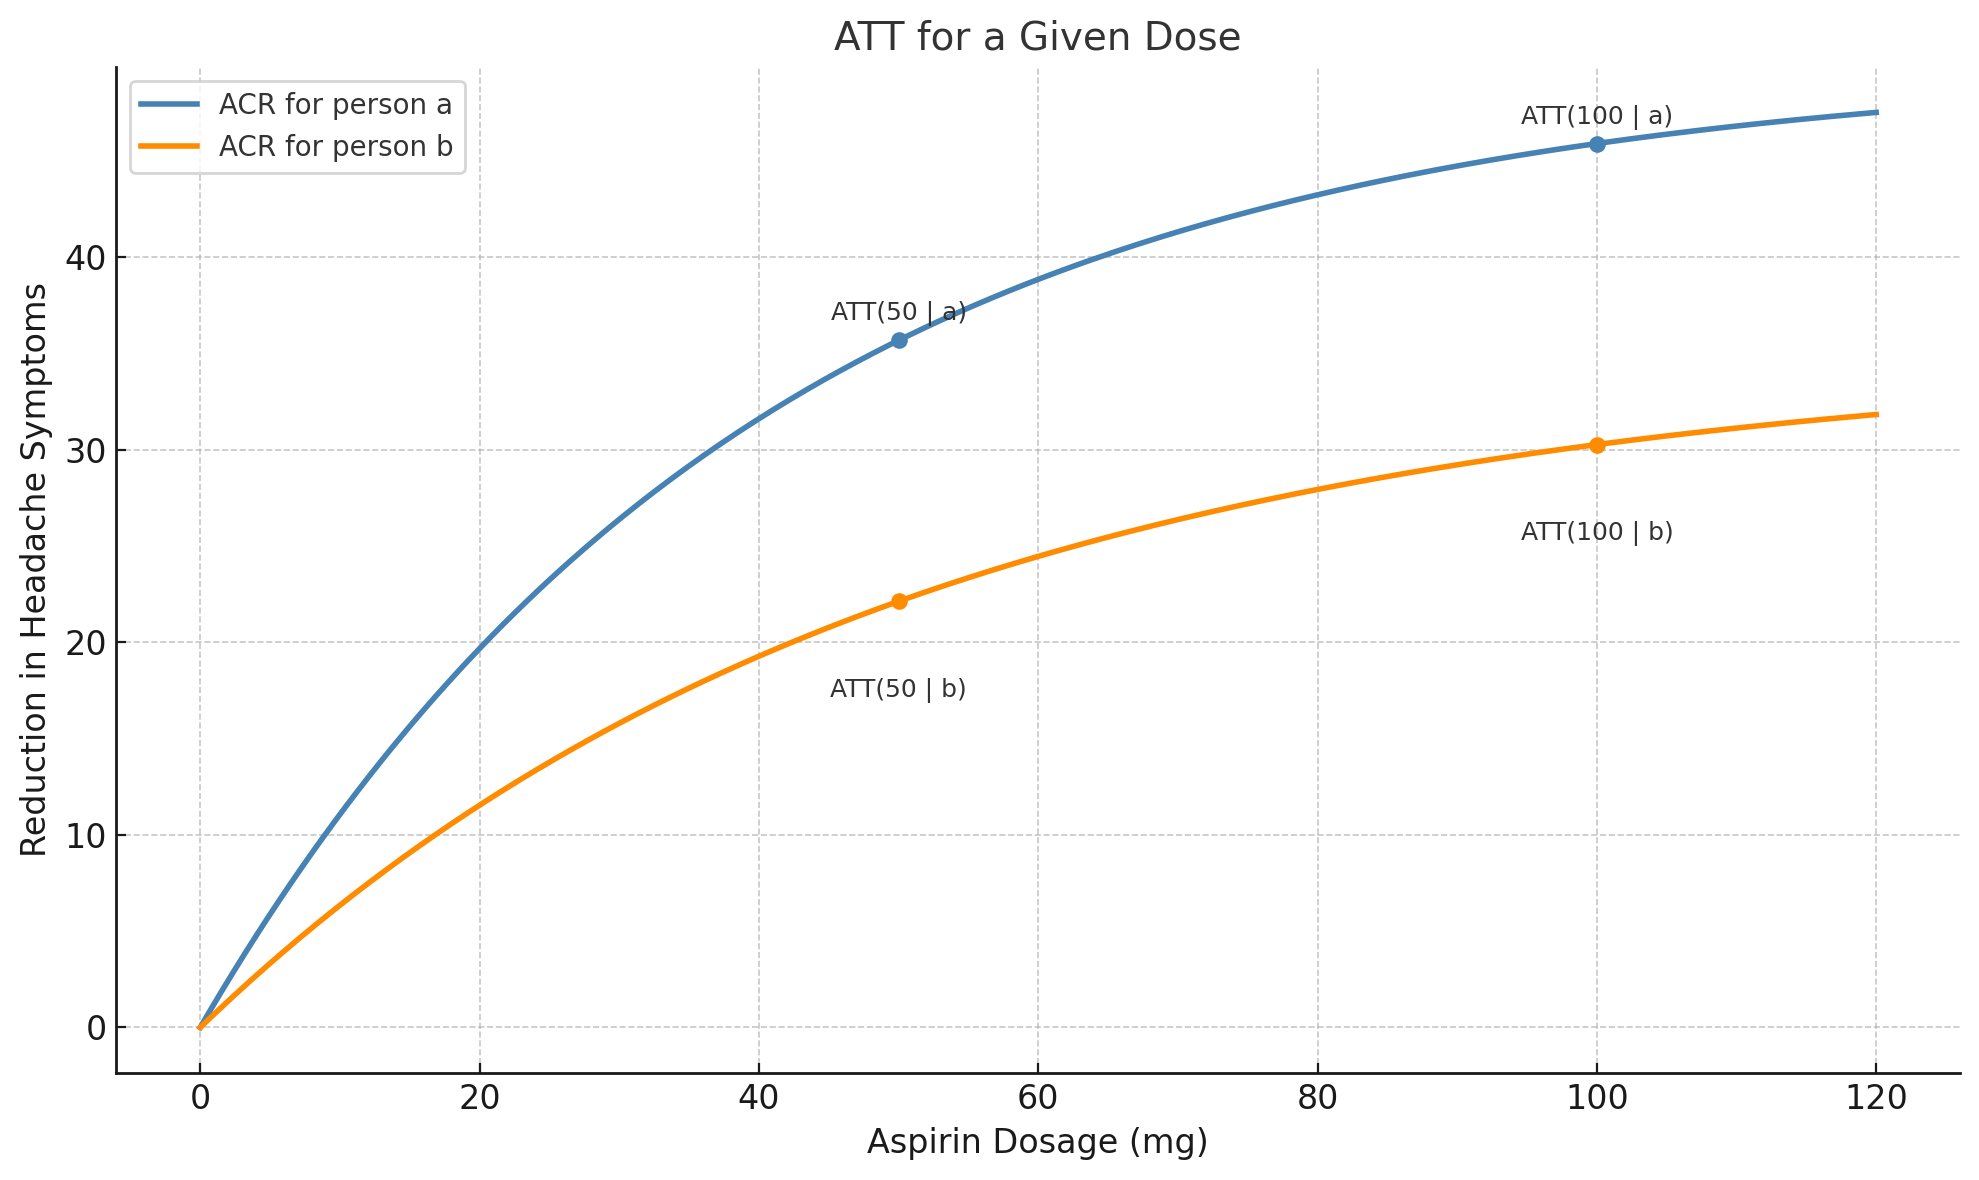
\includegraphics[scale=0.3]{./lecture_includes/acrt_fig2.png}
\end{center}
\end{figure}

What if everyone has different responses?  In other words, Giovanni, person $a$, and Jessica, person $b$, have \emph{difference} causal responses and different \emph{response} at even the same dosage.  Maybe Giovanni responds better to aspirin than Jessica, but Giovanni takes 50 mg, and Jessica takes 100.  What then?

\end{frame}

\begin{frame}{ATT for a given dose}

\begin{figure}
\begin{center}
             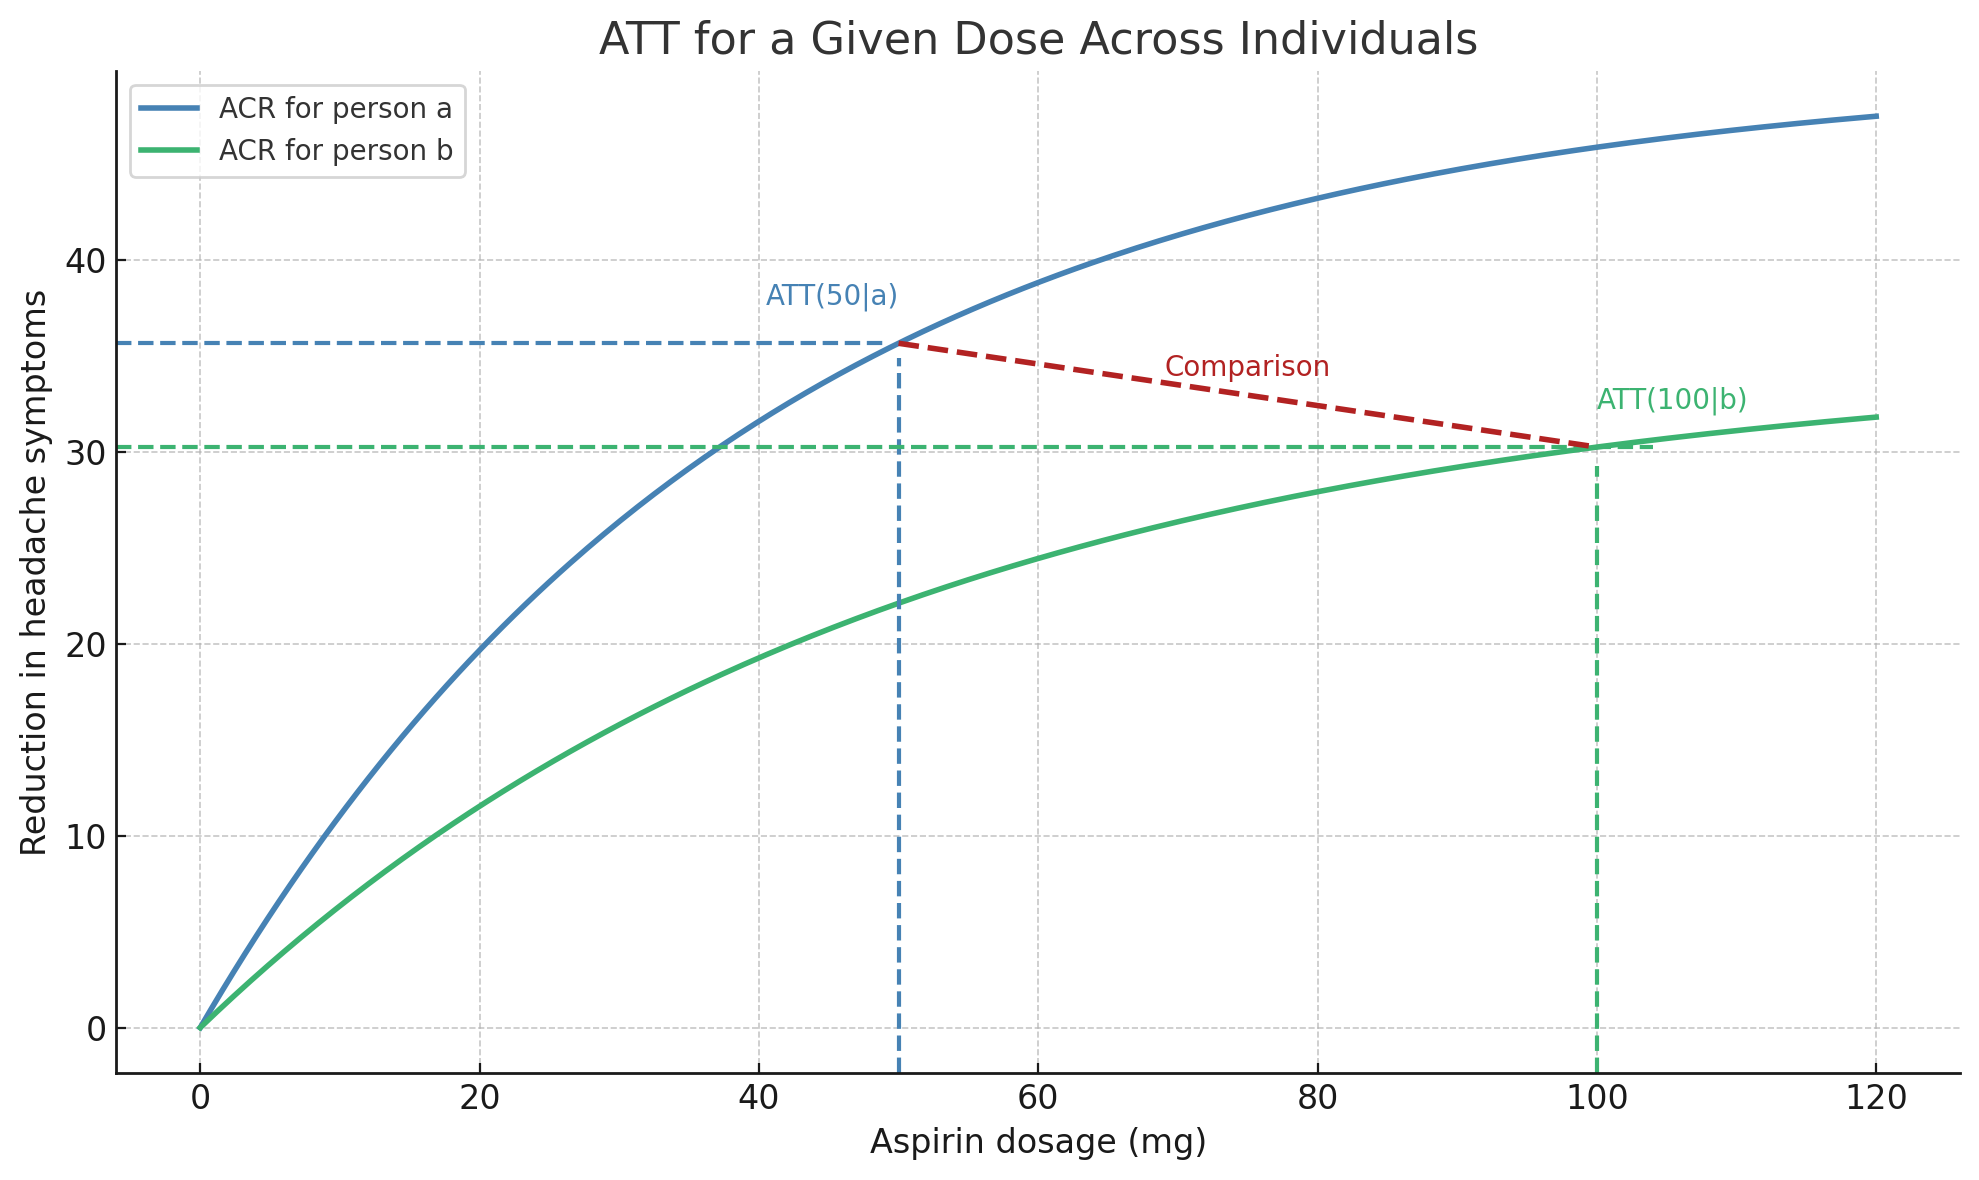
\includegraphics[scale=0.3]{./lecture_includes/acrt_fig2b.png}
\end{center}
\end{figure}

You might estimate negative effects, even though higher dosages actually improve health outcomes

\end{frame}




\begin{frame}{Moving along the dosage is not the ATT}

\begin{itemize}
\item So, the vertical axis is a measure of the ATT(d|d), similar to what we have been doing -- but always the counterfactual is "zero dose"
\item But when if we were to \emph{move} between points?  
\item That's a different parameter called the average causal response for the treated group, or ACRT(d$|$d)
\end{itemize}

\end{frame}
\begin{frame}


\begin{figure}
\begin{center}
             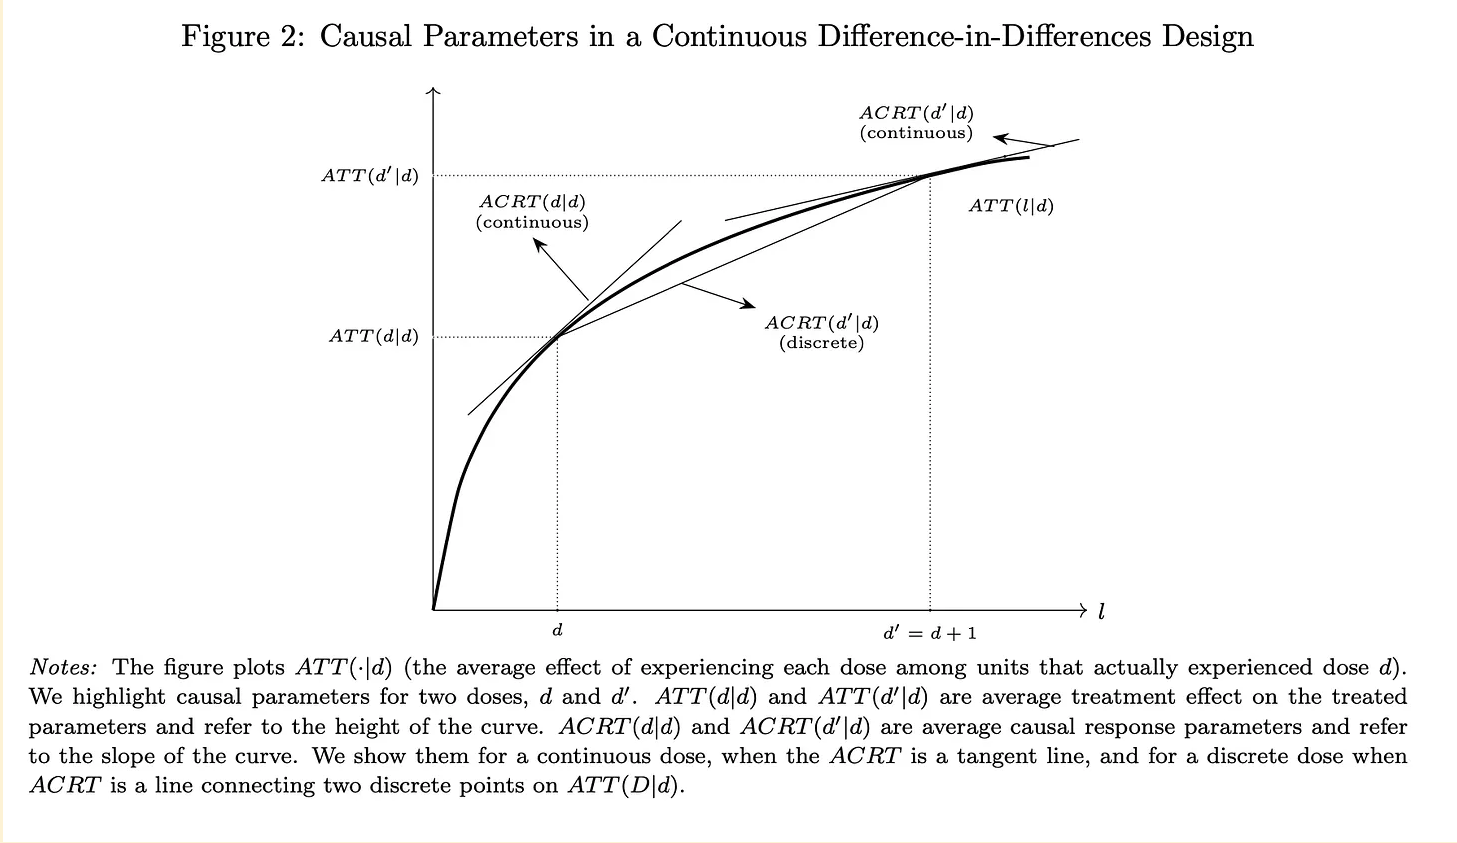
\includegraphics[scale=0.45]{./lecture_includes/continuous1.png}
\end{center}
\end{figure}

\end{frame}

\begin{frame}{What is the ACRT?}

\begin{itemize}
\item ACRT is the causal effect of dose $D=d_j$ vs a different dose $D=D_{j-1}$ for group $d$
	\begin{itemize}
	\item Easiest example is the demand function: at $p=\$10$, I buy 10 units, but at $p=\$11$, I buy 5 units.  
	\item Causal effect of that one dollar increase is $-5$ units
	\item Demand curves are pairs of potential outcomes and treatments and equilibrium ``selects'' one of them
	\end{itemize}
\item Discrete/multi-valued treatment is linear difference between two ATTs for the same city
\item Continuous treatment is the derivative of the function itself
\end{itemize}

\end{frame}

\begin{frame}{Definition of the ACRT}

\begin{figure}
\begin{center}
             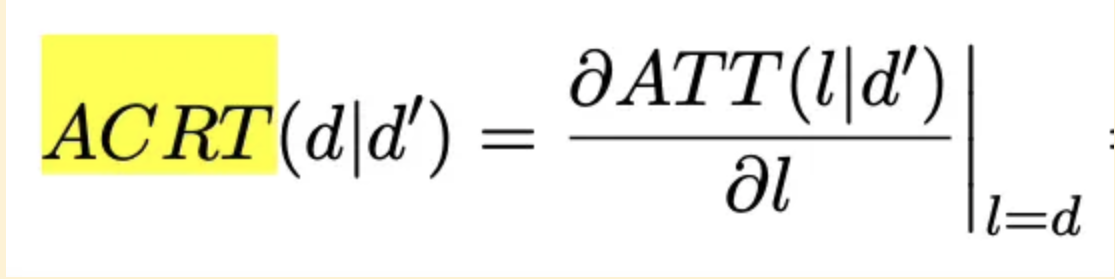
\includegraphics[scale=0.3]{./lecture_includes/continuous4.png}
\end{center}
\end{figure}

\end{frame}



\begin{frame}{Derivation of ACRT}

\begin{figure}
\begin{center}
             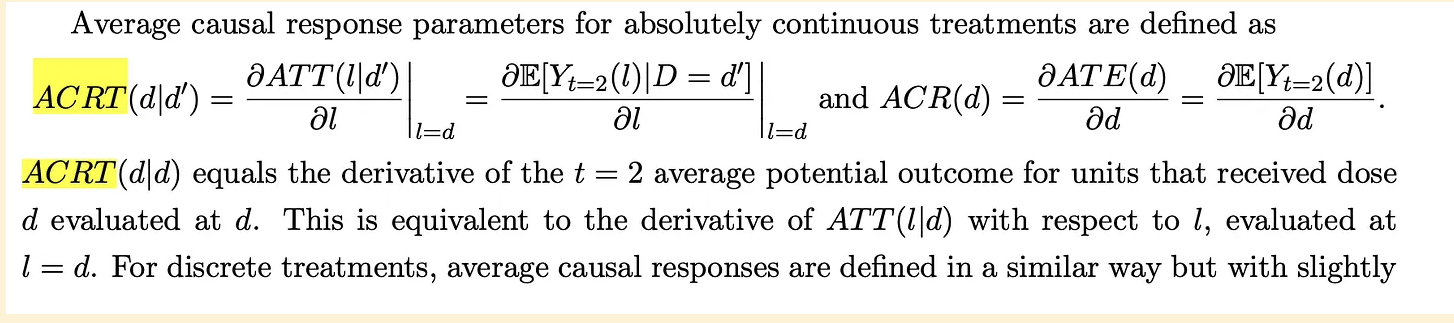
\includegraphics[scale=0.45]{./lecture_includes/continuous2.png}
\end{center}
\end{figure}

\end{frame}
\begin{frame}{Heterogeneities}


\begin{figure}{}
\begin{center}
             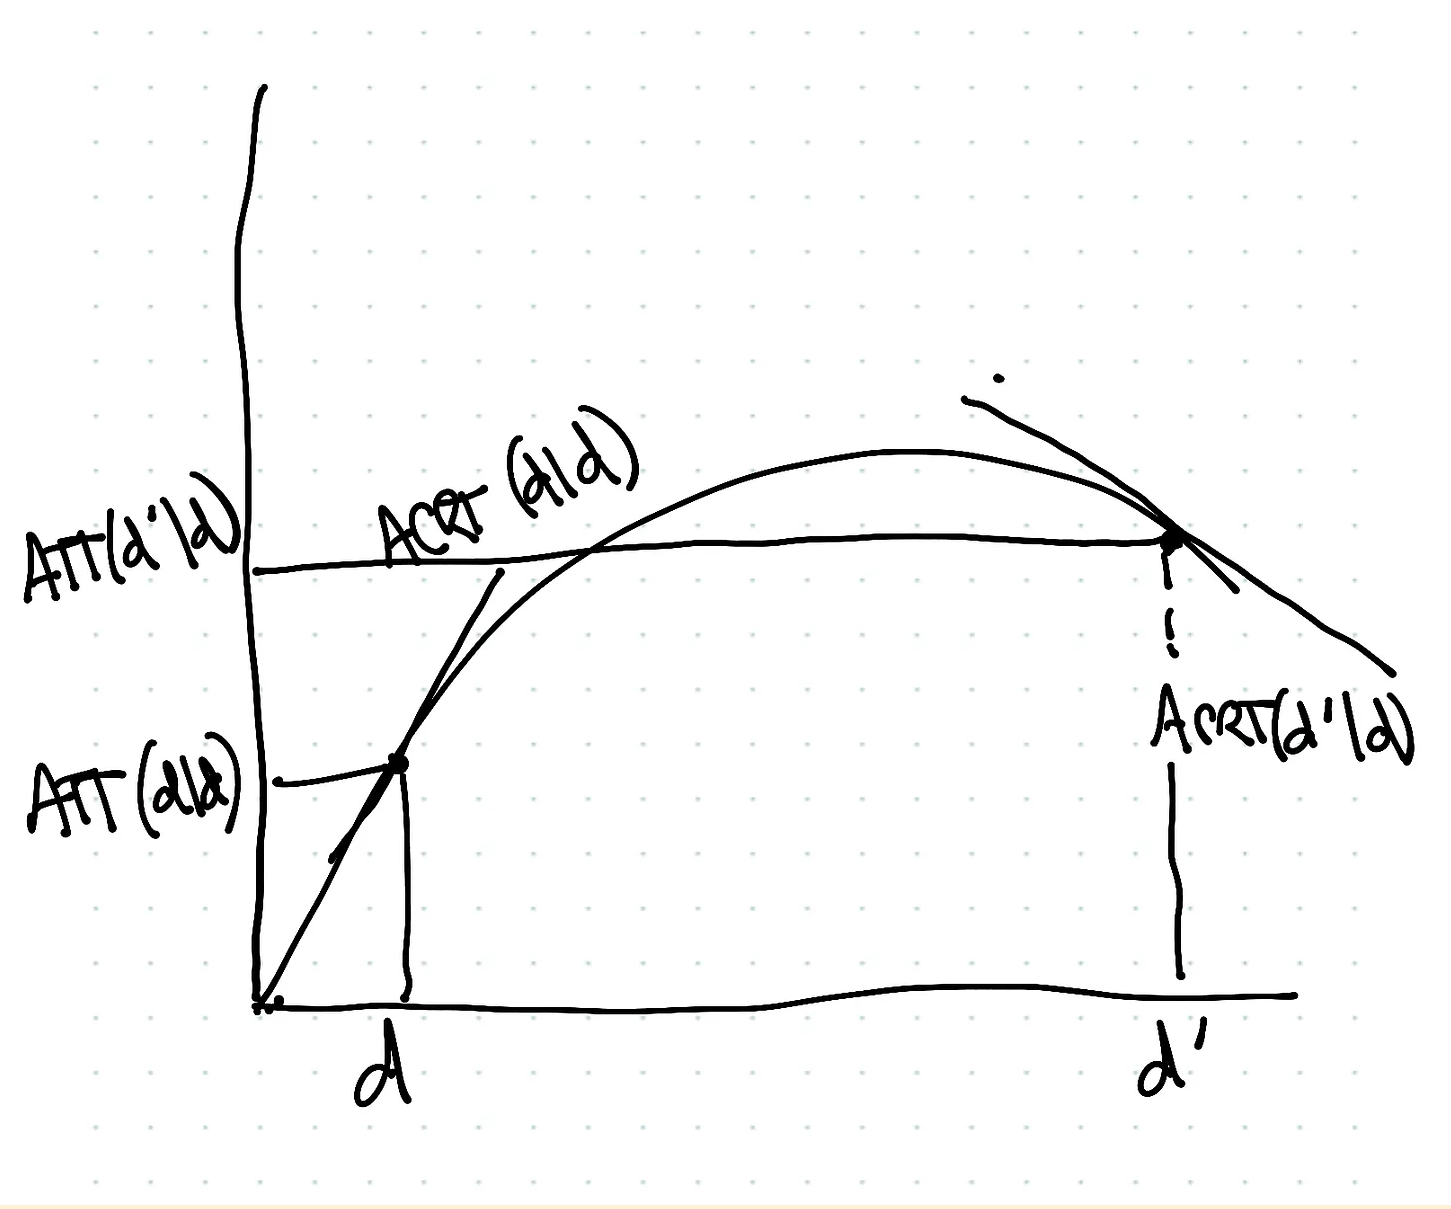
\includegraphics[scale=0.4]{./lecture_includes/continuous3.png}
\end{center}
\end{figure}

\end{frame}








\subsection{Identification}

\begin{frame}{Assumptions}

The authors lay out 5 assumptions, but I’m going to focus on 4. They are:

\begin{enumerate}
\item Random sampling
\item Continuous (2a) and Multi-Valued Treatment (2b)
\item No Anticipation and Observed Outcomes
\item Parallel trends
\end{enumerate}

\end{frame}

\begin{frame}{Identifying $ATT(d|d)$}

We can estimate the $ATT(d|d)$ using the simple DiD equation:

\begin{eqnarray*}
E [ \Delta Y_{it} | D_i = d] - E[ \Delta Y_{it} | D_i = 0]
\end{eqnarray*}

\bigskip

No anticipation and parallel trends converts this comparison of before and after into the $ATT(d|d)$

\bigskip

$ATT(d|d)$ is using as its counterfactual the ``no treatment'', note.  Treatment is a dosage compared to zero iow.

\bigskip

Which means we will need as our controls units whose potential outcome \emph{was always zero} in the long difference

\end{frame}


\begin{frame}{Identifying ACRT}


\begin{eqnarray*}
ATT(b|b) - ATT(a|a) &=& ( E[ \Delta Y_{it} | D_i =a ] - E[ \Delta Y_{it} | D_i = 0]) \\
&& - ( E[ \Delta Y_{it} | D_i =b ] - E[ \Delta Y_{it} | D_i = 0]) \\
&=& E [ \Delta Y_{it} | D_i=a] - E[\Delta Y_{it} | D_i=b]
\end{eqnarray*}

Comparing high and low dose groups.

\end{frame}

\begin{frame}{Identifying ACRT}


\begin{eqnarray*}
ATT(d_j|d_j) - ATT(d_{j-1} | d_{j-1}) &=& \\
( ATT(d_j|d_j) - ATT(d_{j-1} | d_{j}) ) + ( ATT(d_{j-1} | d_j) - ATT(d_{j-1} | d_{j-1}) )&=&  \\
 ( \textcolor{blue}{ACRT(d_j | d_j)} ) + ( \textcolor{red}{ATT(d_{j-1} | d_j) - ATT(d_{j-1} | d_{j-1})} )&=&  \\
\end{eqnarray*}

Part in blue is the movement along the average causal response function, the ACRT, and is causal.  The part in red is selection bias. 

\end{frame}

\begin{frame}{Identifying ACRT}


\begin{eqnarray*}
ATT(d_j|d_j) - ATT(d_{j-1} | d_{j-1}) &=& \\
( ATT(d_j|d_j) - ATT(d_{j-1} | d_{j}) ) + ( ATT(d_{j-1} | d_j) - ATT(d_{j-1} | d_{j-1}) )&=&  \\
 ( \textcolor{blue}{ACRT(d_j | d_j)} ) + ( \textcolor{red}{ATT(d_{j-1} | d_j) - ATT(d_{j-1} | d_{j-1})} )&=&  \\
\end{eqnarray*}

Notice parallel trends allows to identify ATT terms but we need additional assumptions for this red part to vanish. We must assume that the ATT for cities that chose $d_j$ and cities that chose $d_{j-1}$ are the same had they both chose $d_{j-1}$.

\end{frame}

\begin{frame}


\begin{figure}
\begin{center}
             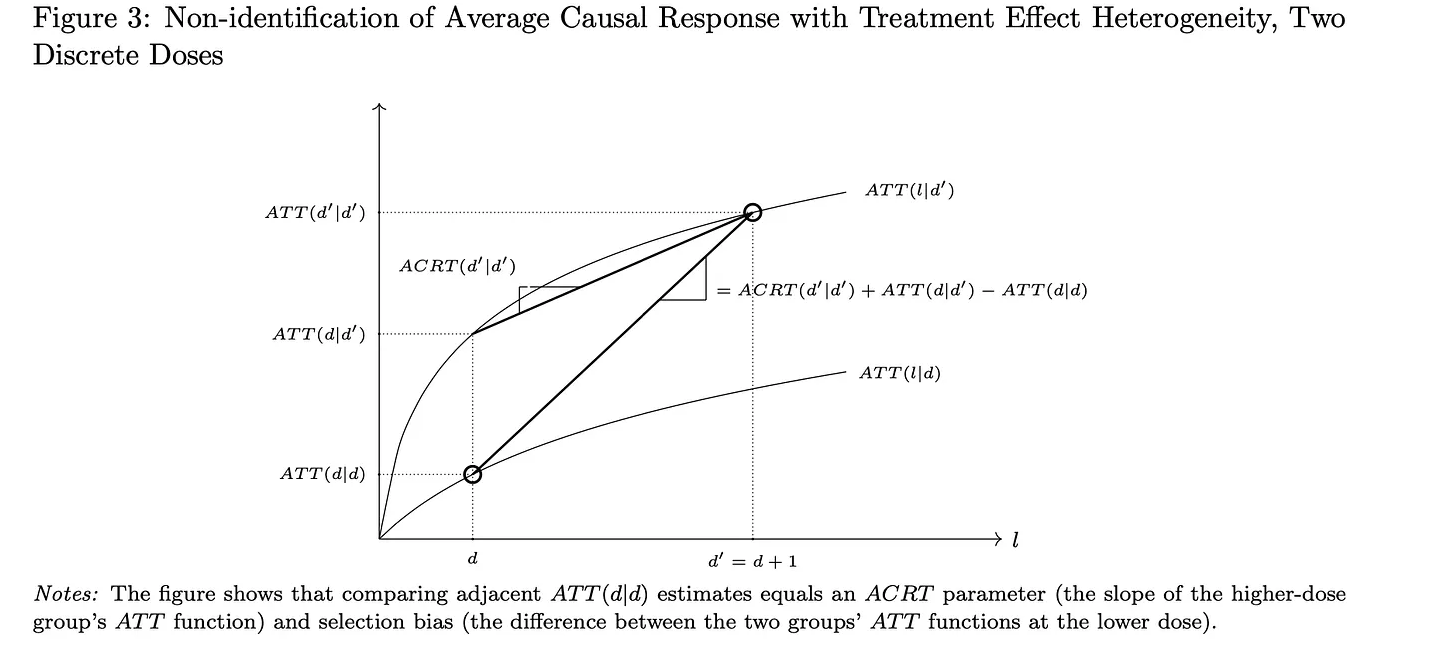
\includegraphics[scale=0.45]{./lecture_includes/continuous5.png}
\end{center}
\end{figure}

\end{frame}

\begin{frame}

\begin{figure}
\begin{center}
             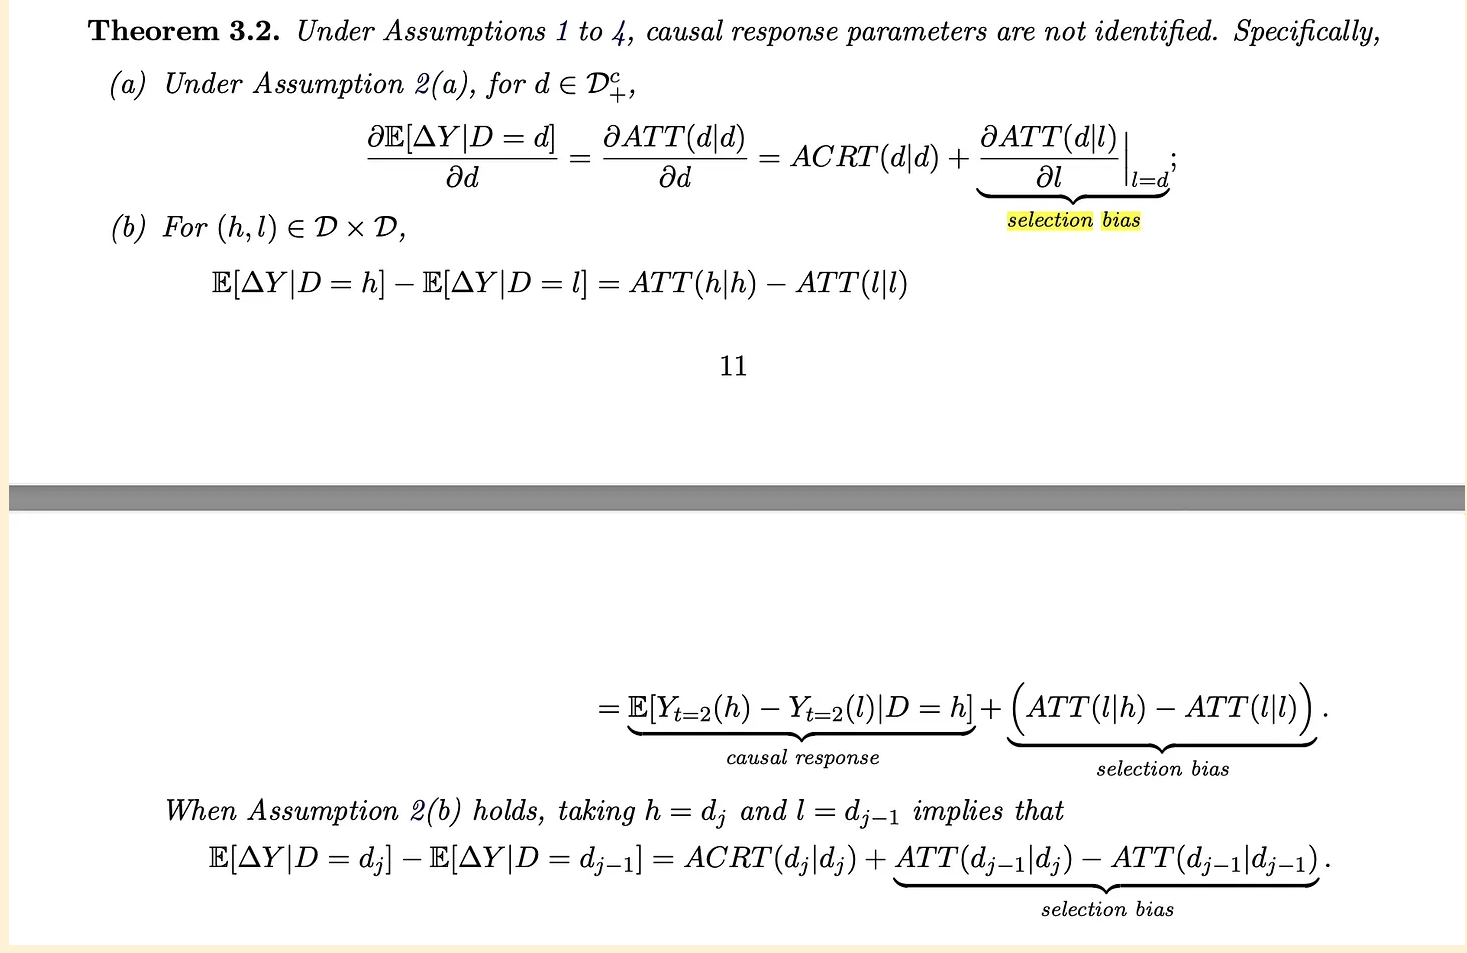
\includegraphics[scale=0.45]{./lecture_includes/continuous6.png}
\end{center}
\end{figure}

\end{frame}

\subsection{Selection bias}



\begin{frame}{Causality and selection bias}

\begin{figure}
\begin{center}
             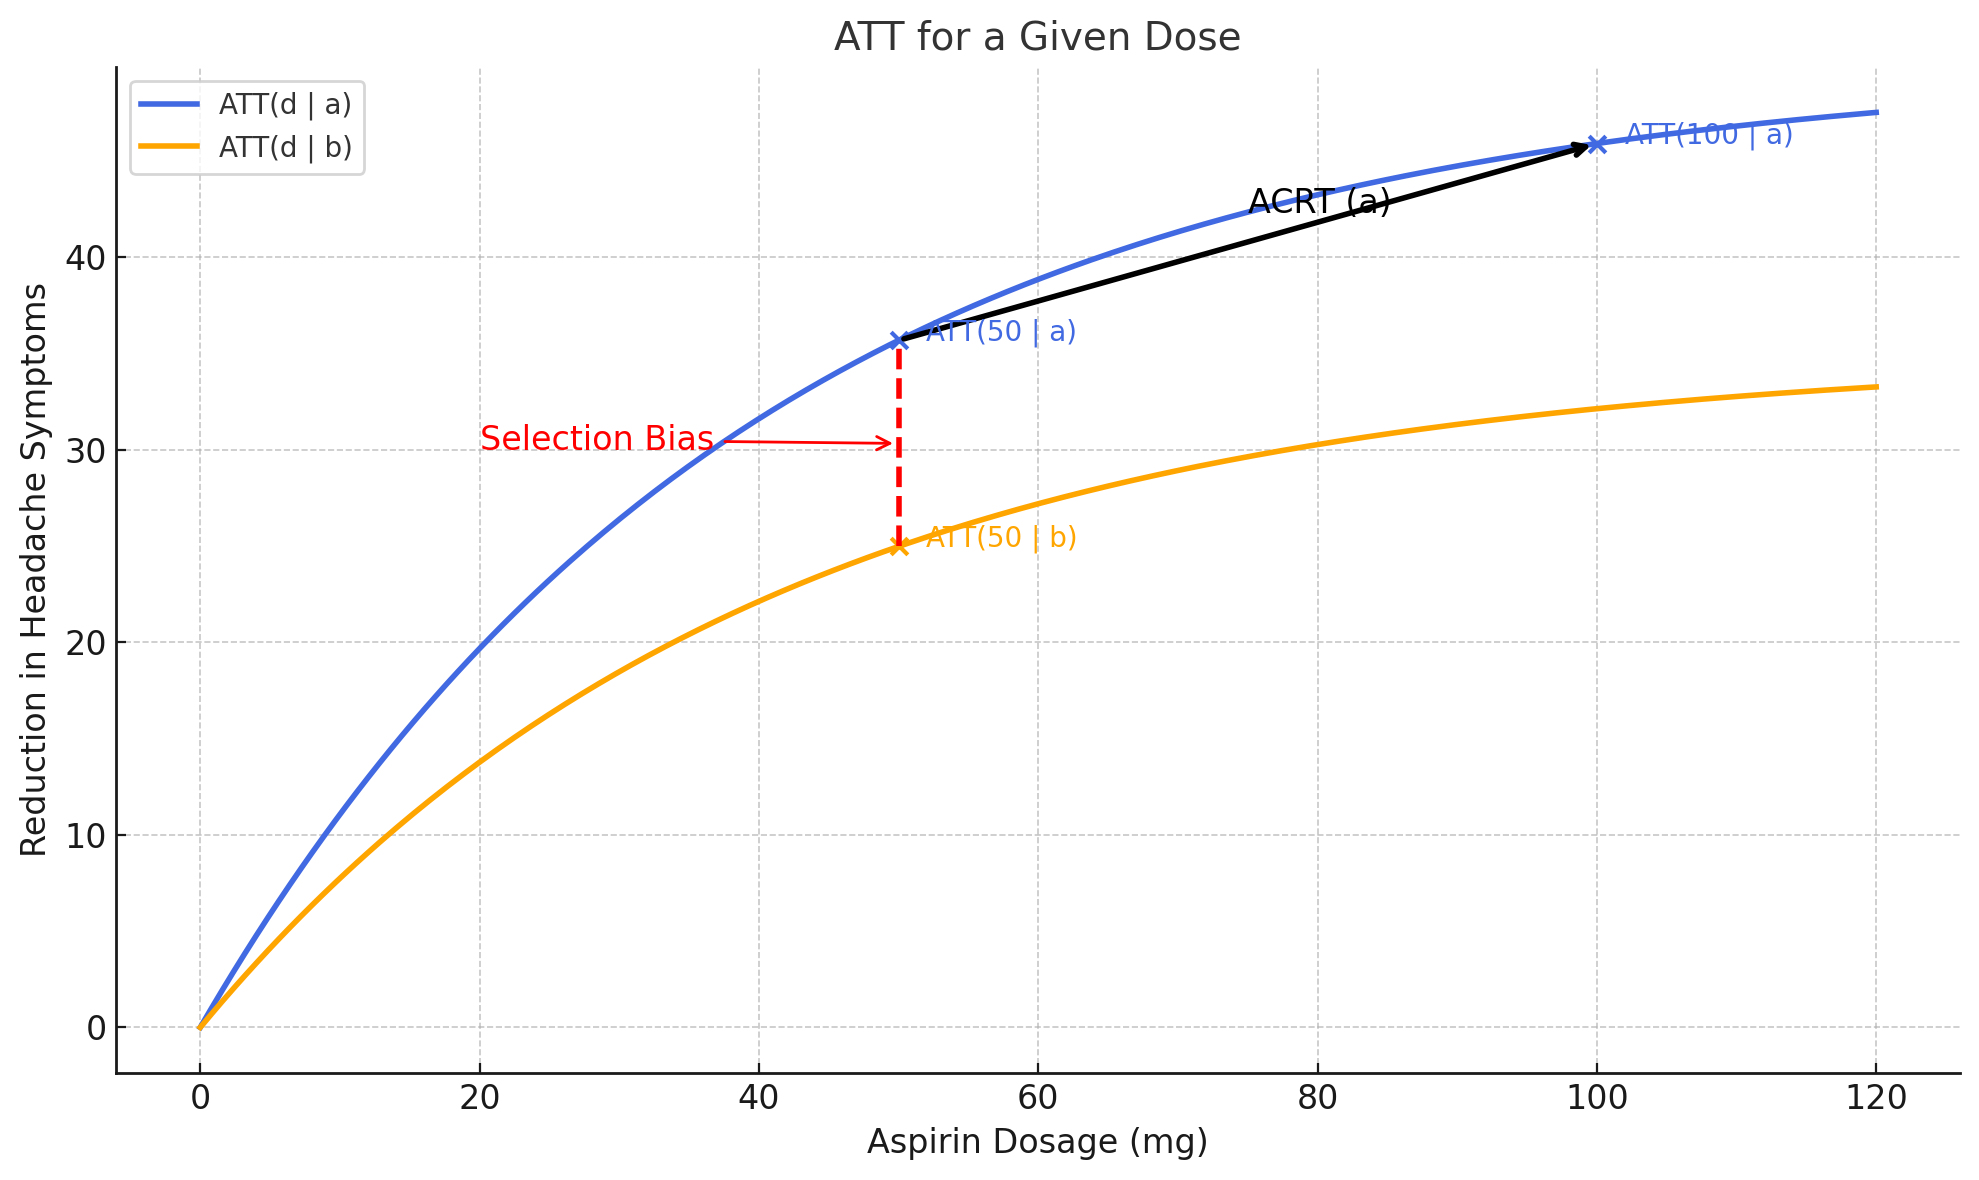
\includegraphics[scale=0.3]{./lecture_includes/acrt_fig2d.png}
\end{center}
\end{figure}

Draw the ACRT for top curve and the selection bias from estimation under assumptions 1 to 4.

\end{frame}


\begin{frame}{Interpreting this}

\begin{itemize}
\item Unrestricted heterogenous treatment effects (across dosage levels and across units with difference dose response functions) is not itself the problem
\item If we randomized dosages, then $\textcolor{red}{ATT(d_{j-1} | d_j) - ATT(d_{j-1} | d_{j-1})}=0$
\item Why?  Because then there is no selection on gains from dosages, and average causal response functions are the same for all dosage groups
\item So then when is this a problem?  Sorting on gains
\end{itemize}

\end{frame}

\begin{frame}{Interpreting this}

\begin{itemize}

\item When estimating treatment effects using continuous DiD, you will need to make one of two assumptions
	\begin{enumerate}
	\item Strong parallel trends: That selection bias isn't there because everyone has the same ACR
	\item Parallel trends plus homogenous treatment effect functions
	\end{enumerate}
\item Roy model like sorting on gains typically lead to violations of the second condition insofar as there is heterogenous returns to dosages across units
\item So the question you have to ask yourself is do you think that cities are ``optimally setting the minimum wage'' around some given minimum wage?
\end{itemize}

\end{frame}

\begin{frame}{Stronger assumption}

\begin{itemize}

\item I'm really not so sure I think that when it comes to state legislation that I think a Roy model is likely responsible for the equilibrium
\item Solving constrained optimization problems is hard and unlikely is it the case that Florida's ATT and Georgia's ATT are terribly different from one another had both chosen the same minimum wage (but that is the bias)
\item Authors introduce a fifth assumption that will eliminate selection bias, but at the price of restricting heterogeneity

\end{itemize}

\end{frame}



\begin{frame}{Discussion of strong parallel trends}

\begin{quote}
We discuss an alternative but typically stronger assumption, which we call strong parallel trends, that says that the path of outcomes for lower-dose units must reflect how higher-dose units’ outcomes would have changed had they instead experienced the lower dose. Thus, strong parallel trends restricts treatment effect heterogeneity and justifies comparing dose groups. Absent this type of condition, comparisons across dose groups include causal responses but are “contaminated” by an additional term involving possibly different treatment effects of the same dose for different dose groups—we refer to this additional term as selection bias.
\end{quote}

\end{frame}

\begin{frame}{A5: Strong parallel trends}

\begin{figure}
\begin{center}
             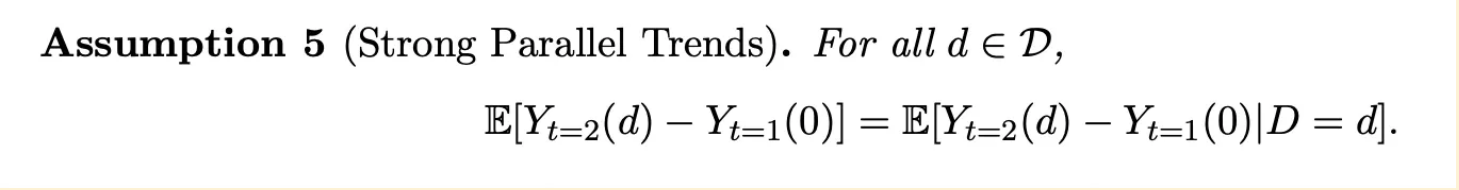
\includegraphics[scale=0.45]{./lecture_includes/continuous7.png}
\end{center}
\end{figure}

\end{frame}


\begin{frame}{Randomization and strong parallel trends}

\begin{itemize}

\item Randomized dosages guarantees that the ACRT are the same across all dosage groups
\item In this situation, strong parallel trends holds because all dosages have the same ATE and ACRT
\item Roy like sorting on dosage may be the biggest challenge you'll face -- schooling stops, family size may not satisfy strong parallel trends

\end{itemize}

\end{frame}






\subsection{Interpreting TWFE}

\begin{frame}{Interpreting TWFE results}

\begin{figure}
\begin{center}
             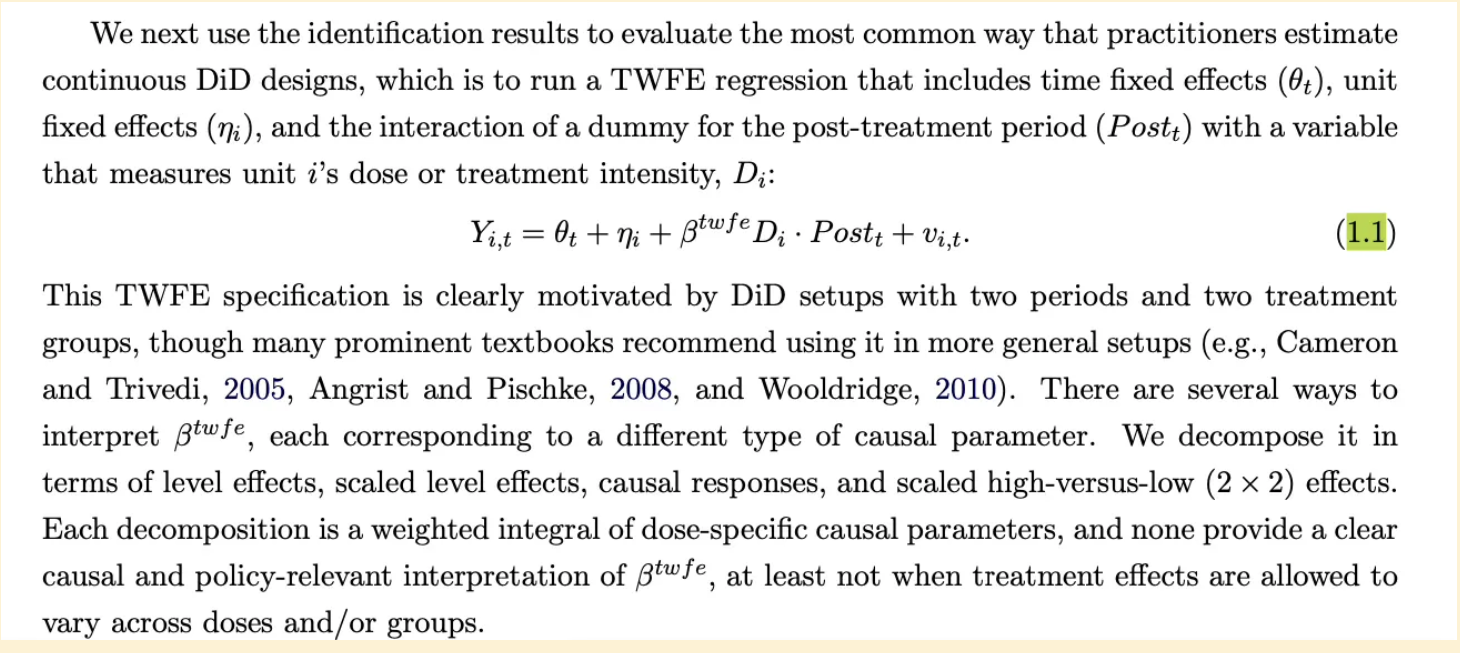
\includegraphics[scale=0.45]{./lecture_includes/continuous8.png}
\end{center}
\end{figure}

\end{frame}


\begin{frame}

\begin{figure}
\begin{center}
             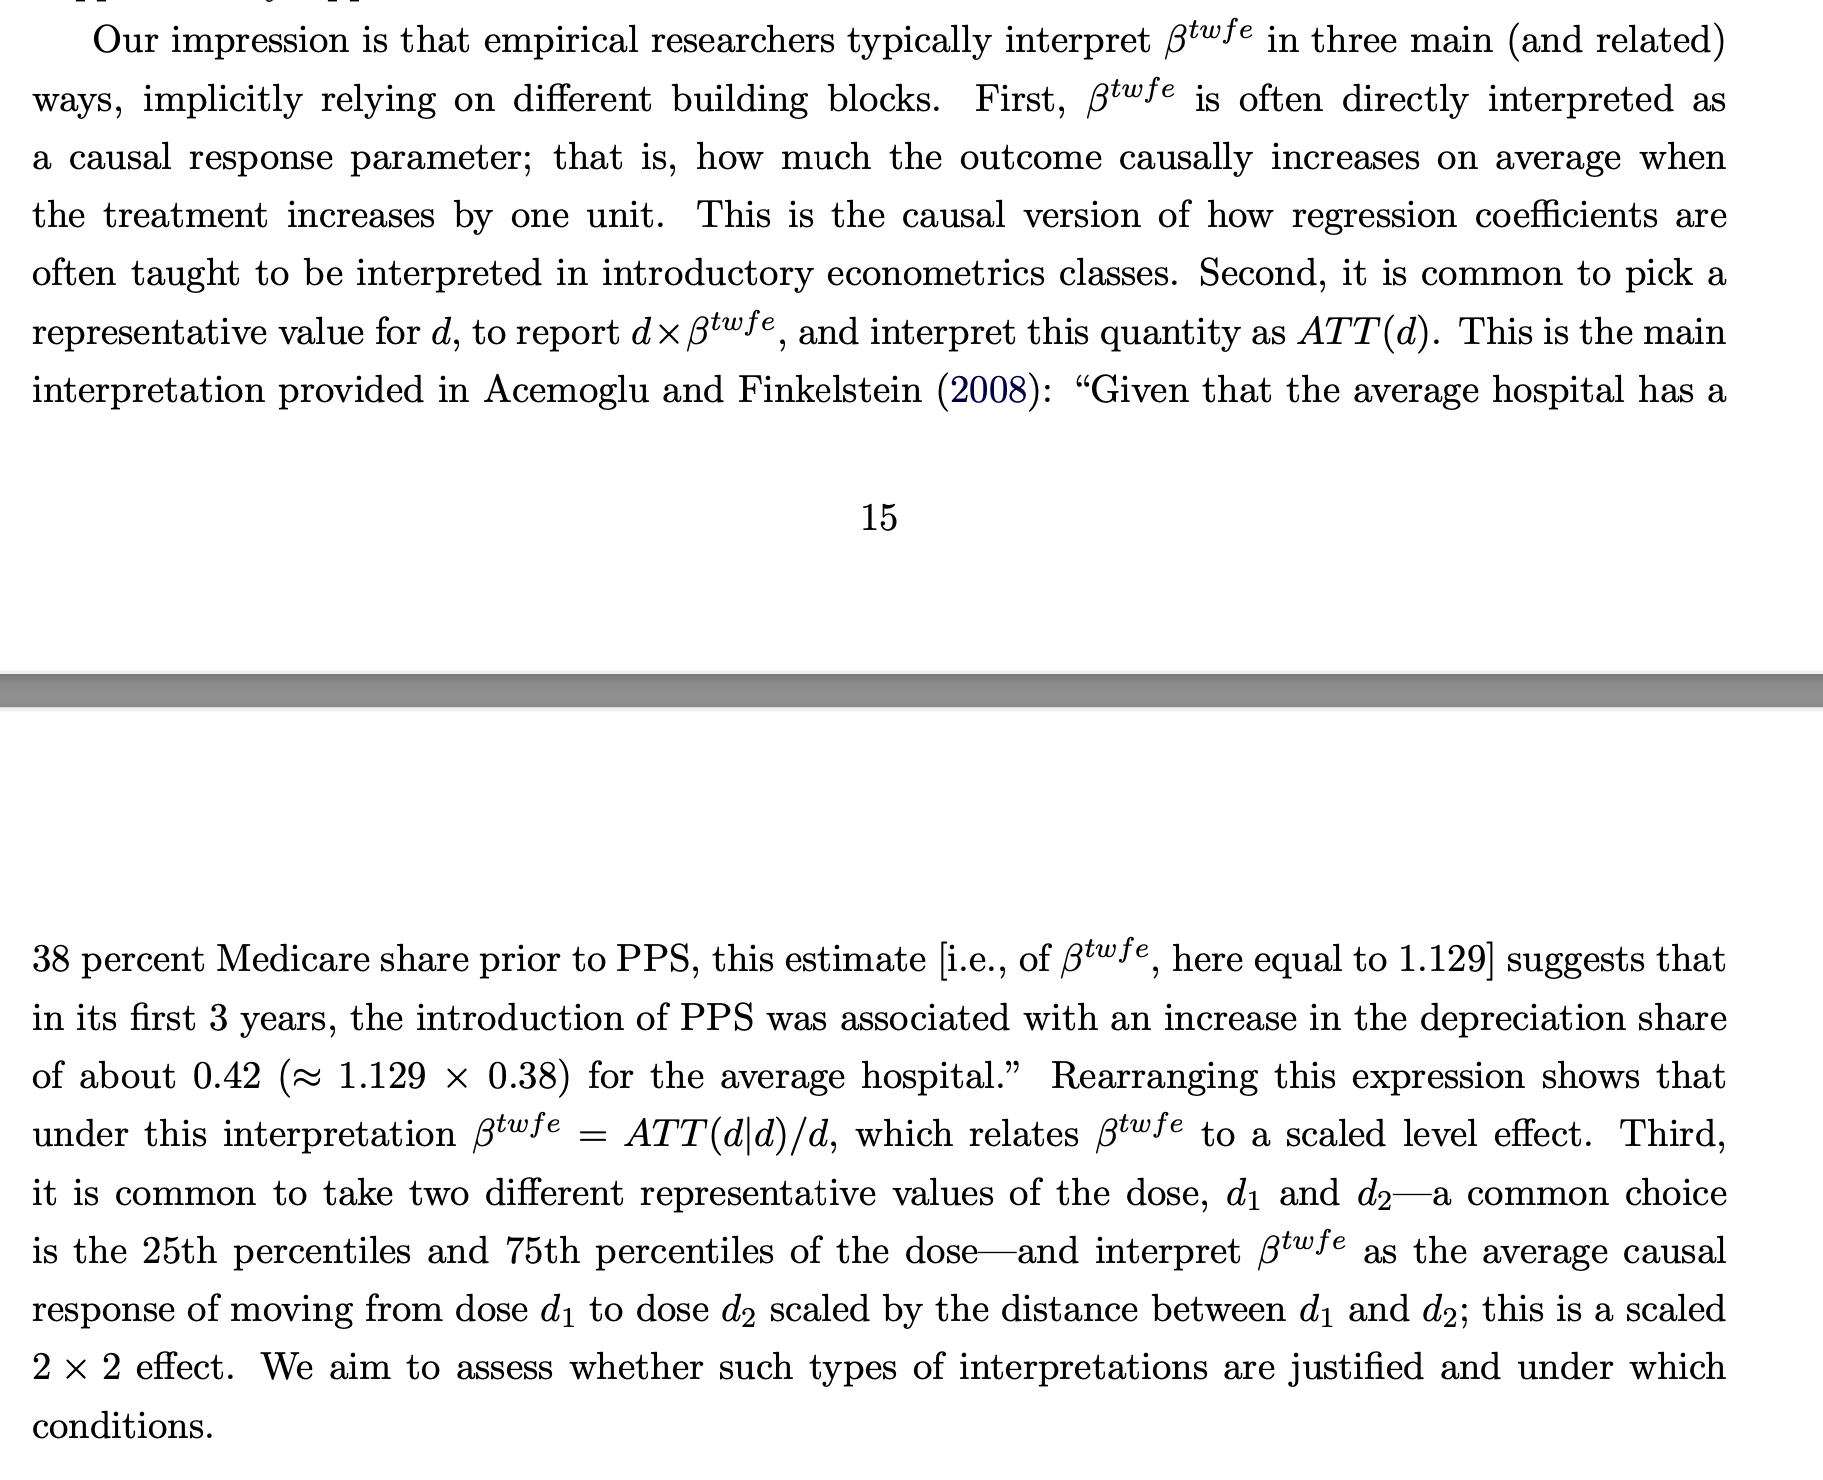
\includegraphics[scale=0.35]{./lecture_includes/continuous12.png}
\end{center}
\end{figure}

\end{frame}





\begin{frame}{Interpreting TWFE}

\begin{figure}
\begin{center}
             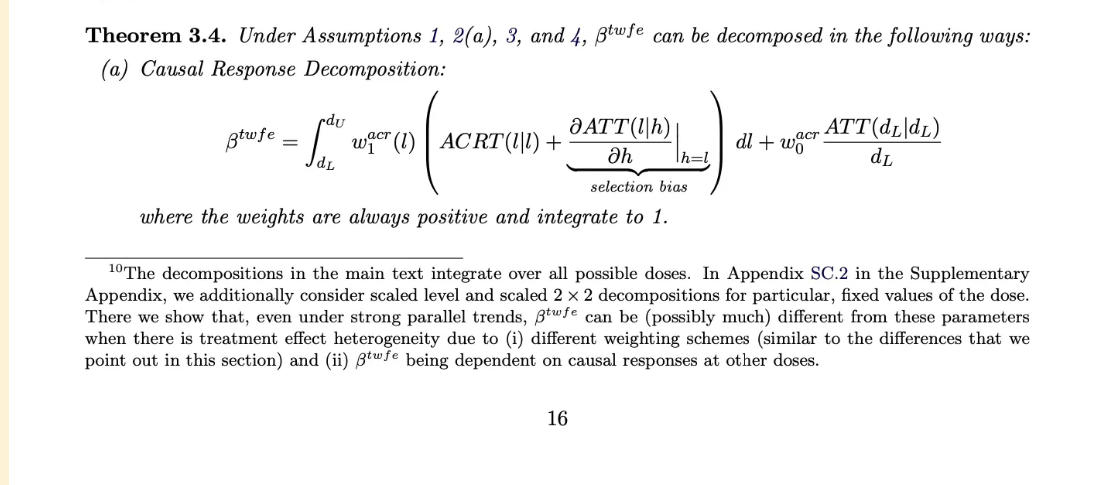
\includegraphics[scale=0.55]{./lecture_includes/continuous9.png}
\end{center}
\end{figure}

\end{frame}


\begin{frame}

\begin{figure}
\begin{center}
             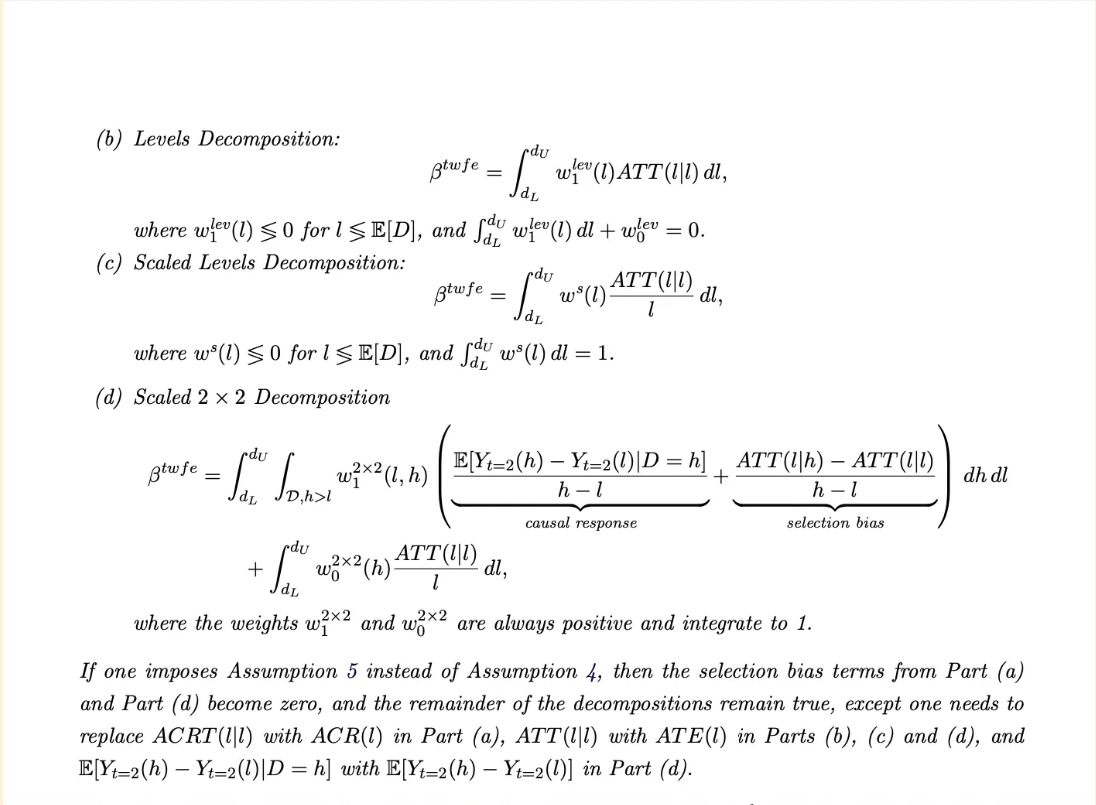
\includegraphics[scale=0.5]{./lecture_includes/continuous10.png}
\end{center}
\end{figure}

\end{frame}
\begin{frame}

\begin{figure}
\begin{center}
             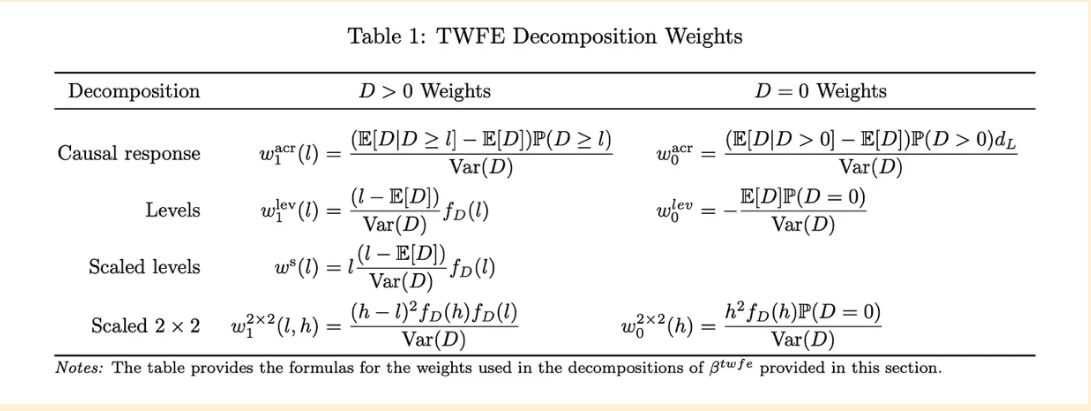
\includegraphics[scale=0.5]{./lecture_includes/continuous11.png}
\end{center}
\end{figure}

\end{frame}








\begin{frame}
\frametitle{Understanding Decomposition Results}

\begin{itemize}
  \item The pattern from decomposition shows distinct impacts of parameter types.
  \item \textbf{Level-effect parameters} (parts b and c):
    \begin{itemize}
      \item $\beta_{twfe}$ is not influenced by selection bias.
      \item Includes negative weights.
    \end{itemize}
  \item \textbf{Comparative doses parameters} (parts a and d):
    \begin{itemize}
      \item $\beta_{twfe}$ carries positive weights.
      \item Encounters selection bias under parallel trends.
    \end{itemize}
\end{itemize}
\end{frame}


\begin{frame}
\frametitle{Addressing Selection Bias and Weighting Schemes}

\begin{itemize}
  \item Parametric linearity restrictions may overlook weighting scheme issues inherent in TWFE regression.
  \item These restrictions do not resolve selection bias problems.
  \item Next, we explore:
    \begin{itemize}
      \item Alternative estimators to TWFE that adjust the weighting scheme.
      \item These alternatives do not rely on the stringent linearity assumption.
      \item Selection bias issues persist and require different solutions.
    \end{itemize}
\end{itemize}
\end{frame}

\section{Estimation and an Example}

\begin{frame}{Institutional Background — Texas House Bill 2 (HB2)}

\begin{itemize}
\item In July 2013, Texas passed HB2, imposing new regulations on abortion providers.
\item Two provisions had major impact:
	\begin{enumerate}
	\item Required physicians to have admitting privileges at a hospital within 30 miles of the clinic.
	\item Required clinics to meet ambulatory surgical center (ASC) standards.
	\end{enumerate}
\item The admitting privileges rule went into effect on November 1, 2013, forcing nearly half of the state’s clinics to close.
\item This caused large increases in travel distance and congestion at remaining clinics.
\end{itemize}

\end{frame}


\begin{frame}{Clinic Access Map}

\begin{center}
  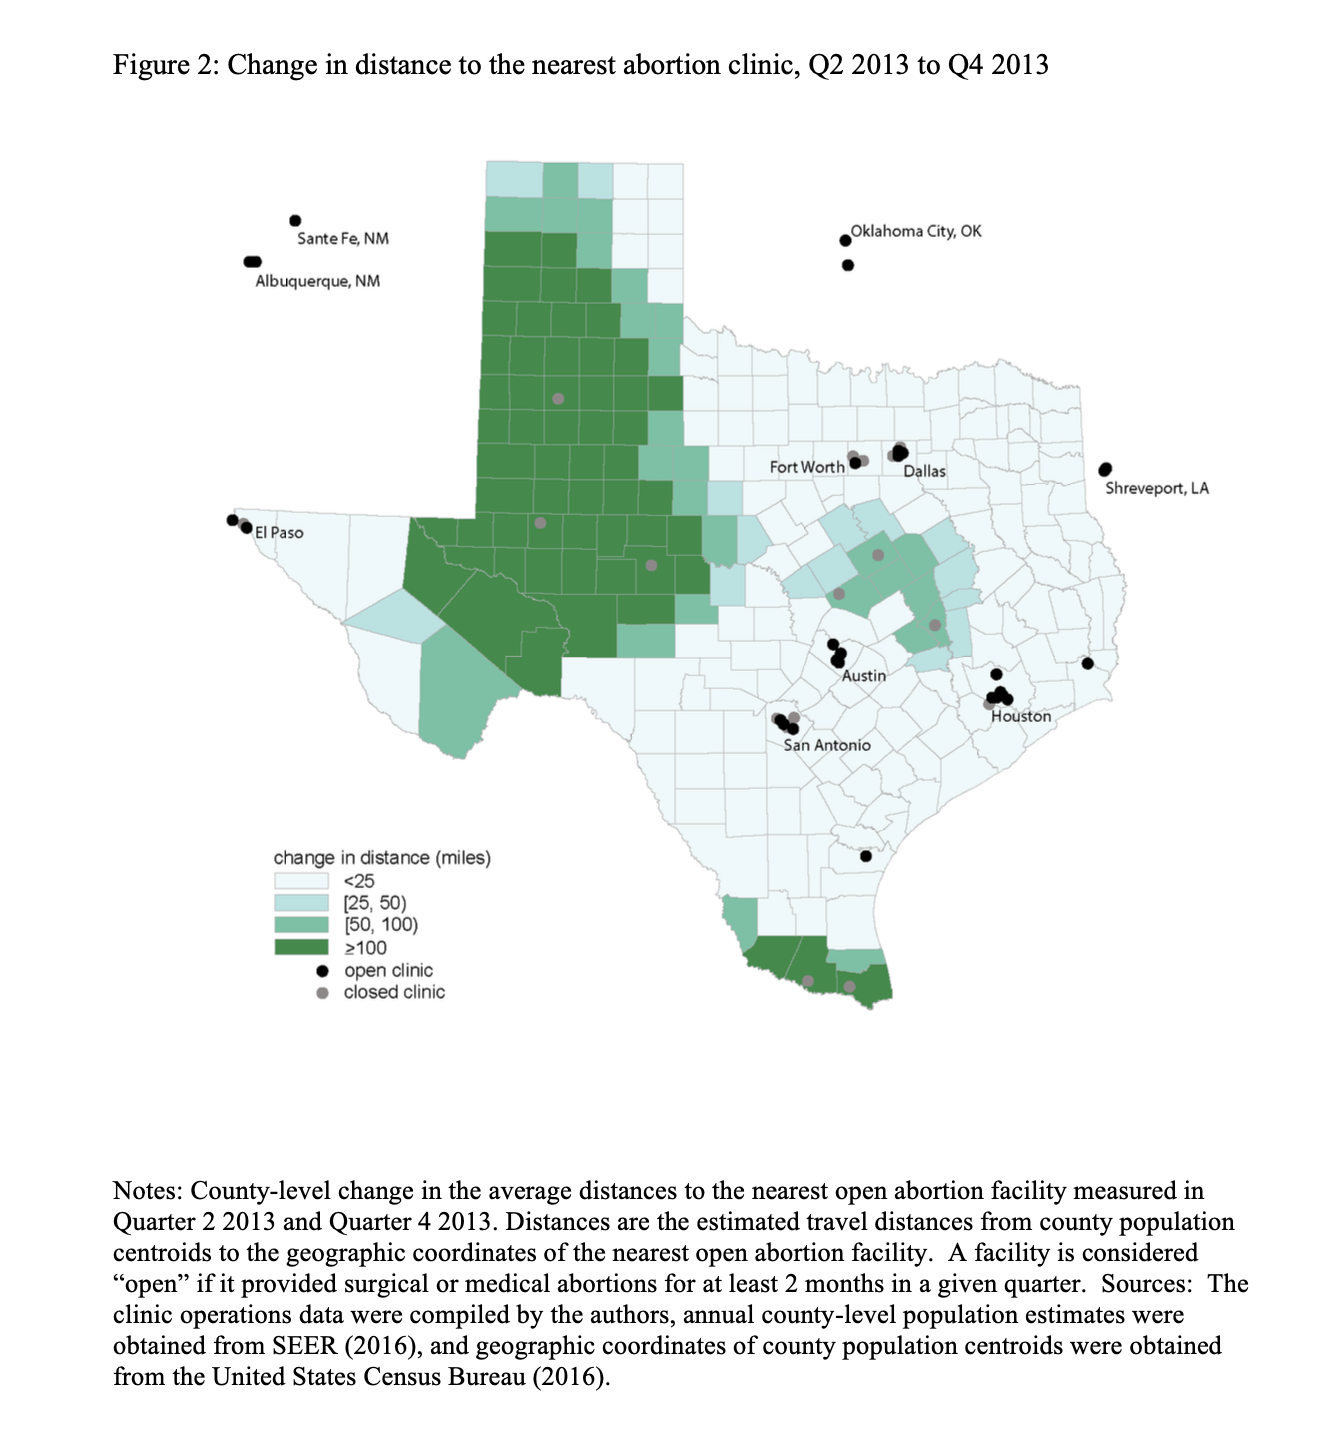
\includegraphics[width=0.9\linewidth]{./lecture_includes/abortion_map.png}
\end{center}

\end{frame}



\begin{frame}{Our Poisson Fixed Effects Model}

We estimate a generalized DiD using Poisson pseudo-likelihood:
\[
\mathbb{E}[Y_{ct} \mid D_{ct}, X_{ct}, \alpha_c, \lambda_t] = \exp(\beta D_{ct} + \alpha_c + \lambda_t + \gamma X_{ct})
\]

\begin{itemize}
  \item $Y_{ct}$: Count of abortions per county-year (age-standardized).
  \item $D_{ct}$: Distance bin indicators and average service population.
  \item $\alpha_c$, $\lambda_t$: County and year fixed effects.
  \item $X_{ct}$: Controls (demographics, unemployment, family planning access).
\end{itemize}

\medskip

\end{frame}

\begin{frame}{Main Results}

\textbf{Key Findings (Table 2, Column 1):}
\begin{itemize}
  \item 50–100 miles $\rightarrow$ \textbf{16\% reduction} in abortion rates
  \item 100–150 miles $\rightarrow$ \textbf{28\% reduction}
  \item $>$200 miles $\rightarrow$ \textbf{44\% reduction}
  \item +100,000 in service population $\rightarrow$ \textbf{7\% reduction}
\end{itemize}

\medskip

\textbf{Interpretation:}
\begin{itemize}
  \item Both distance and clinic congestion significantly reduce access.
  \item Effects are non-linear—biggest impact occurs at shorter distances.
  \item Congestion explains more than half the overall effect of clinic closures.
\end{itemize}

\end{frame}

\begin{frame}{Estimating $\text{ATT}(d \mid d)$ from Clinic Closures}

Now we want to estimate the causal effect of clinic closures on abortion rates, allowing that effect to vary with dose $d$ — where dose = distance to nearest clinic.

\medskip

We'll estimate a \textbf{dose-specific DiD}, defined as:
\[
  \widehat{\text{ATT}}(d \mid d) = \mathbb{E}[\Delta Y_i \mid D_i = d] - \mathbb{E}[\Delta Y_i \mid D_i = 0]
\]

\begin{itemize}
  \item The second term is the average change in abortion rates in counties with no clinic closures.
  \item The first term is the average change in counties with exposure $D_i = d$.
  \item We're not using Poisson here — we'll estimate this directly using nonparametric methods from CGBS (2024).
\end{itemize}

\end{frame}



\begin{frame}{Step 1: Binning the Dose (Distance)}

A simple approach is to group counties by their post-HB2 distance to the nearest open clinic.

\medskip

Within each bin, we compute the average change in abortion rates:
\[
\widehat{\text{ATT}}(\text{bin}) = \mathbb{E}[\Delta Y_i \mid D_i \in \text{bin}] - \mathbb{E}[\Delta Y_i \mid D_i = 0]
\]

\begin{itemize}
  \item This gives us a discrete approximation of ATT(d|d) at several key exposure levels.
  \item We would then show those visually
\end{itemize}

\end{frame}


\begin{frame}{Estimating $\text{ATT}(d \mid d)$ via Binned DiD}

Let’s start with a simple idea: divide counties by their \textbf{dose} — i.e., the post-HB2 distance to the nearest clinic.

\bigskip

For each bin of distance $B$, estimate the causal effect of clinic closure exposure on abortion rates:

\[
\widehat{\text{ATT}}(B \mid B) = \mathbb{E}[\Delta Y_i \mid D_i \in B] - \mathbb{E}[\Delta Y_i \mid D_i = 0]
\]

\begin{itemize}
  \item $\Delta Y_i = Y_{i1} - Y_{i0}$ is the change in abortion rates in county $i$.
  \item Control group: counties with $D_i = 0$ (no change in access).
  \item Treated group: counties with $D_i$ in bin $B$.
\end{itemize}

\end{frame}



\begin{frame}{Step-by-Step: What Do We Do?}

\textbf{Step 1: Define bins of distance}

\begin{itemize}
  \item Bin 1: 0–50 miles
  \item Bin 2: 50–100 miles
  \item Bin 3: 100–150 miles
  \item Bin 4: 150–200 miles
  \item Bin 5: $>$200 miles
\end{itemize}

\bigskip

\textbf{Step 2: For each bin, construct a dummy:}
\[
\text{Treated}_i = 1\{D_i \in \text{Bin } B\}
\]

\textbf{Step 3: Subset the data to:}
\begin{itemize}
  \item Units with $D_i \in B$ (treated) and
  \item Units with $D_i = 0$ (control)
\end{itemize}

\end{frame}




\begin{frame}{Step-by-Step: Estimation per Bin}

\textbf{Step 4: Estimate the DiD}

\[
\Delta Y_i = \alpha + \beta_B \cdot \text{Treated}_i + \varepsilon_i
\]

\begin{itemize}
  \item $\Delta Y_i$ is the change in outcome (e.g., abortion rate) from pre- to post-period.
  \item $\text{Treated}_i = 1$ if $D_i$ is in bin $B$, 0 if $D_i = 0$.
  \item $\beta_B$ estimates $\text{ATT}(B \mid B)$ for bin $B$.
\end{itemize}

\bigskip

\textbf{Repeat this process} for each bin to get a full set of ATT estimates across the dose distribution.

\end{frame}




\begin{frame}{Why This Works (and When It Doesn’t)}

\textbf{Why this is valid:}
\begin{itemize}
  \item Relies only on standard parallel trends: untreated units represent the counterfactual trend.
  \item No functional form assumptions on dose response.
\end{itemize}

\bigskip

\textbf{Limitations:}
\begin{itemize}
  \item Requires sufficient untreated and treated units per bin.
  \item Bin definitions can affect results.
  \item Flat effects within bins — no curvature captured.
\end{itemize}

\end{frame}




\begin{frame}{Binned Estimation: Pros and Cons}

\textbf{Advantages:}
\begin{itemize}
  \item Easy to explain and plot: good for papers and policy presentations.
  \item Lets us see effect heterogeneity across dose levels.
\end{itemize}

\bigskip

\textbf{Disadvantages:}
\begin{itemize}
  \item Estimates are “flat” within each bin.
  \item Shape depends on bin cutpoints — can be misleading if dose-response is smooth.
\end{itemize}

\end{frame}


\begin{frame}{Alternative Method: Smoothed Estimation of $\text{ATT}(d \mid d)$}

As an alternative to binning, we use a smoothed estimator of $\text{ATT}(d \mid d)$.

\bigskip

This method is based on work by Chen, Christensen, and Kankanala (2023), and adapted to the difference-in-differences setting by Callaway, Goodman-Bacon, and Sant’Anna (2024).


\end{frame}


\begin{frame}{Alternative Method: Smoothed Estimation of $\text{ATT}(d \mid d)$}

\textbf{Key idea:}
\begin{itemize}
  \item Smoothly estimate $\mathbb{E}[\Delta Y_i \mid D_i = d]$ across dose levels using only treated units ($D_i > 0$)
  \item Subtract off $\mathbb{E}[\Delta Y_i \mid D_i = 0]$ from untreated counties
\end{itemize}

\[
\widehat{\text{ATT}}(d \mid d) = \widehat{\mathbb{E}}[\Delta Y_i \mid D_i = d] - \widehat{\mathbb{E}}[\Delta Y_i \mid D_i = 0]
\]

This gives a continuous estimate of treatment effects across the dose distribution.

\end{frame}




\begin{frame}{Intuition and Implementation with \texttt{condid}}

\textbf{What the method does (intuitively):}
\begin{enumerate}
  \item Calculate $\Delta Y_i = Y_{i,\text{post}} - Y_{i,\text{pre}}$ for each county
  \item For treated units ($D_i > 0$), regress $\Delta Y_i$ on a flexible function of $D_i$ (e.g., B-splines)
  \item Predict $\mathbb{E}[\Delta Y_i \mid D_i = d]$ across the observed dose range
  \item Subtract the average change in untreated units ($D_i = 0$)
\end{enumerate}


\end{frame}

\begin{frame}{Intuition and Implementation with \texttt{condid}}

We’ll implement this using the \texttt{condid} package in R, developed by Brantly Callaway.

\begin{itemize}
  \item Includes built-in routines for smoothed $\text{ATT}(d \mid d)$ estimation
  \item \textbf{Currently does not support covariates}, but is actively being expanded
\end{itemize}

\end{frame}



\begin{frame}
\frametitle{Implementation and Parameters}

\textbf{Treatment Assignment:}
\begin{itemize}
    \item $D_i = $ distance increase from 2013 to 2014 if $> 10$ miles, 0 otherwise
    \item $G_i = $ 2014 if treated, 0 if never-treated (control)
    \item 126 counties treated, 128 counties control
\end{itemize}

\end{frame}


\begin{frame}
\frametitle{Implementation and Parameters}

\textbf{Key Parameters:}
\begin{align}
ATT(d|d) &= \mathbb{E}[Y_t(d) - Y_t(0) | D=d] \\
ACRT(d|d) &= \frac{\partial ATT(l|d)}{\partial l}\Big|_{l=d} \\
ACRT^o &= \mathbb{E}[ACRT(D|D) | D>0]
\end{align}


\end{frame}


\begin{frame}
\frametitle{Implementation and Parameters}


\textbf{Interpretation:}
\begin{itemize}
    \item $ATT(d|d)$: Effect of dose $d$ vs. no treatment for counties that got dose $d$
    \item $ACRT(d|d)$: Dose-response curve connecting all ATT points (under strong PT)
    \item $ACRT^o$: Overall average marginal effect (single coefficient in output)
    \item Allows heterogeneous effects across dose levels
\end{itemize}

\vspace{0.3cm}

\textbf{Identification:} Parallel trends between treated and never-treated counties

\end{frame}







\end{document}

\begin{frame}{$\text{ATT}(d \ | \ d)$ estimators}
  In general, the $\text{ATT}(d \ | \ d)$ estimators will take the form of
  $$
    \expechat{\Delta Y_i}{D_i = d} - \expechat{\Delta Y_i}{D_i = 0}
  $$

  \begin{itemize}
    \item The second term is just the average change in $Y$ from the control group

    \item The first-term is where we have some options
  \end{itemize}
\end{frame}

\begin{frame}{Option 1: Bins}
  The simplest procedure is to `discretize' doses into a set of bins

  \bigskip
  Then, form a DID estimate for each bin
\end{frame}

\imageframe{lecture_includes/continuous_did/continuous_binned_avgs.pdf}

\begin{frame}{Pros and Cons of Bins}
  Advantges:
  \begin{itemize}
    \item Creates a discrete set of groups that are easy to discuss in your paper

    \item Event-studies are easy to estimate (one for each bin)
  \end{itemize}

  \bigskip
  Disadvantages:
  \begin{itemize}
    \item Bins create a flat surface that is likely not perfectly specified (but gets close as the number of bins grow)
  \end{itemize}
\end{frame}

\begin{frame}{Option 2: Non-parametric smoothing}
  Alternatively, $\expechat{\Delta Y_i}{D_i = d}$ can be estimated with non-parametric methods

  \bigskip
  The simplest way is to use non-parametric method on $\Delta Y_i - \expechat{\Delta Y_i}{D_i = 0}$ with only the $D_i > 0$ observations.
  \begin{itemize}
    \item The result of this will be the DID estimates

    \item Standard errors produced should be correct (can always bootstrap to be safe)
  \end{itemize}
\end{frame}

\imageframe{lecture_includes/continuous_did/continuous_smoothed_avgs.pdf}

\begin{frame}{Pros and Cons of Non-parametric smoothing}
  Advantges:
  \begin{itemize}
    \item Better estimates the smooth evolution of $\expechat{\Delta Y_i}{D_i = d}$
  \end{itemize}

  \bigskip
  Disadvantages:
  \begin{itemize}
    \item Event-studies are hard to display (one plot for each event-time?)
  \end{itemize}
\end{frame}





\end{document}

\begin{frame}{Switching to a lab}

\begin{itemize}

\item We'll first look at my friend's lecture notes from CodeChella Madrid and go through his code in Stata
\item Then I'm going to go through my abortion clinic paper and \emph{attempt} to see if I did it!

\end{itemize}

\end{frame}

\subsection{Continuous valued dose}

\begin{frame}{Doctor example extended}
  Now, let's say we have a continuous distribution of doses
  \begin{itemize}
    \item Some units receive 0mg
    \item Others receive some amount between 0 and 20mg
  \end{itemize}
\end{frame}

\imageframe{lecture_includes/continuous_did/continuous_raw_first_differences.pdf}

\begin{frame}{Dose-specific DID estimates}
  Our previous method of having dose-specific DID estimates will be quite noisy in this setting
  \begin{itemize}
    \item Very few individuals with the \emph{same} dose

    \item Throwing out information of individuals with very similar dose
  \end{itemize}
\end{frame}

\imageframe{lecture_includes/continuous_did/continuous_did_estimates.pdf}

\begin{frame}{Alternative strategies}
  Our previous strategy clearly will not suffice

  \bigskip
  An alternative strategy is to \emph{pool} observations with similar doses to estimate an average $\expec{\Delta Y_i}{D_i = d}$
  \begin{itemize}
    \item E.g. say you break doses into 2mg bins (0--2, 2--4, etc.) and take averages in those bins

    \item Or any other of your favorite non-parametric method for estimating
  \end{itemize}
\end{frame}

\begin{frame}{$\text{ATT}(d \ | \ d)$ estimators}
  In general, the $\text{ATT}(d \ | \ d)$ estimators will take the form of
  $$
    \expechat{\Delta Y_i}{D_i = d} - \expechat{\Delta Y_i}{D_i = 0}
  $$

  \begin{itemize}
    \item The second term is just the average change in $Y$ from the control group

    \item The first-term is where we have some options
  \end{itemize}
\end{frame}

\begin{frame}{Option 1: Bins}
  The simplest procedure is to `discretize' doses into a set of bins

  \bigskip
  Then, form a DID estimate for each bin
\end{frame}

\imageframe{lecture_includes/continuous_did/continuous_binned_avgs.pdf}

\begin{frame}{Pros and Cons of Bins}
  Advantges:
  \begin{itemize}
    \item Creates a discrete set of groups that are easy to discuss in your paper

    \item Event-studies are easy to estimate (one for each bin)
  \end{itemize}

  \bigskip
  Disadvantages:
  \begin{itemize}
    \item Bins create a flat surface that is likely not perfectly specified (but gets close as the number of bins grow)
  \end{itemize}
\end{frame}

\begin{frame}{Option 2: Non-parametric smoothing}
  Alternatively, $\expechat{\Delta Y_i}{D_i = d}$ can be estimated with non-parametric methods

  \bigskip
  The simplest way is to use non-parametric method on $\Delta Y_i - \expechat{\Delta Y_i}{D_i = 0}$ with only the $D_i > 0$ observations.
  \begin{itemize}
    \item The result of this will be the DID estimates

    \item Standard errors produced should be correct (can always bootstrap to be safe)
  \end{itemize}
\end{frame}

\imageframe{lecture_includes/continuous_did/continuous_smoothed_avgs.pdf}

\begin{frame}{Pros and Cons of Non-parametric smoothing}
  Advantges:
  \begin{itemize}
    \item Better estimates the smooth evolution of $\expechat{\Delta Y_i}{D_i = d}$
  \end{itemize}

  \bigskip
  Disadvantages:
  \begin{itemize}
    \item Event-studies are hard to display (one plot for each event-time?)
  \end{itemize}
\end{frame}


\section{Empirical Example}

\begin{frame}{Lu and Yu, 2015}
  This example will use data from
  ``Trade Liberalization and Markup Dispersion: Evidence from China's WTO Accession'' (Lu and Yu, American Economic Journal: Applied Economics 2015)
\end{frame}

\begin{frame}{China's WTO Ascension}
  The paper uses the entrance of China into the World Trade Organization (WTO) in 2002

  \bigskip
  When entering the WTO, tariffs at the industry level were expected to drop to at most 10\%
\end{frame}

\begin{frame}{Defining continuous treatment variable}
  The research strategy is to compare industries (at the 3-digit SIC level) that had higher or lower pre-existing tariff rates

  \begin{itemize}
    \item After the entrance in 2002, industries with higher tariff had \emph{larger} decreases in tariffs $\implies$ a larger shock in import competition
  \end{itemize}

  \bigskip
  Can define treatment as
  $D_i = \max (0, \text{Tariff}_{2001} - 0.10)$
  \begin{itemize}
    \item How much tariffs are expected to drop
  \end{itemize}
\end{frame}

\begin{frame}{Outcome variable: Markup Dispersion}
  The dataset is an industry-by-year panel dataset
  \begin{itemize}
    \item Each row is an industry in China in a given year
  \end{itemize}

  \bigskip
  The outcome variable is the industry-level \emph{Theil Markup Index}, which measures how much spread in markups at the firm level
  \begin{itemize}
    \item Higher markup index $\implies$ less competitive market
  \end{itemize}

  \pause
  \bigskip
  \textbf{Hypothesis:} Larger decrease in tariffs $\implies$ more competition $\implies$ decrease in markup dispersion
\end{frame}

\begin{frame}{$2 \times 2$ setup}
  We will use 2000 ($t = 0$) and 2004 ($t = 1$) as our initial years

  \bigskip
  Let's look at the raw data
  \begin{itemize}
    \item $x$-axis is our treatment vairable $D_i = \max (0, \text{Tariff}_{2001} - 0.10)$

    \item $y$-axis is the change in markup dispersion $\Delta \ln \text{Theil}_i = \ln \text{Theil}_{i, 2004} - \ln \text{Theil}_{i, 2000}$
  \end{itemize}
\end{frame}

\imageframe{lecture_includes/continuous_did/china_wto_raw.pdf}

\begin{frame}{Parallel Trends assumption}
  Our identification assumption is that if China did not enter the WTO, counterfactual changes in markup dispersion is the same for the unaffected group and the affected doses

  \begin{itemize}
    \item We can assess the plausability using pre-periods (later)
  \end{itemize}

  \pause
  \bigskip\bigskip
  To estimate counterfactual trend, we will take average $\Delta \ln \text{Theil}_i$ for the $D_i = 0$ group
\end{frame}

\imageframe{lecture_includes/continuous_did/china_wto_raw.pdf}

\imageframe{lecture_includes/continuous_did/china_wto_ests.pdf}

\begin{frame}{Pre-trends `test'}
  Redo the previous estimates using
  $$
    \Delta \ln \text{Theil}_i = \ln \text{Theil}_{i, 1998} - \ln \text{Theil}_{i, 2000}
  $$

  \bigskip
  We are hoping that the pre-trend change in markup dispersion is uncorrelated with the dose received, $D_i$
\end{frame}

\imageframe{lecture_includes/continuous_did/china_wto_pretrends_ests.pdf}






\begin{frame}{TWFE has many meanings}

\begin{itemize}

\item Today I just wanted to emphasize the basic principles though -- define the parameter, figure out the assumptions, then build the estimators
\item Just running regressions doesn't work once we have heterogenous treatment effects
\item ``Although strong parallel trends removes the selection bias, the weights attached to the causal parameters are still hard to interpret''
\item New papers have developed new methods experimenting with different assumptions, but still waiting on the software
\end{itemize}

\end{frame}




\end{document}






\end{document}



\section{Fuzzy DiD}





\begin{frame}{Sharp DiD}

\begin{itemize}
\item In a ``sharp'' DiD, a group gets treated in period 1, a control group does not
\item Parallel trends allows you to identify ATT
\item We discussed several methods
\item But sometimes the lines between treatment and control groups get ``fuzzy''
\end{itemize}

\end{frame}

\begin{frame}{Fuzziness}

\begin{itemize}
\item In a ``fuzzy'' DiD design, there's growth in treatment occurring among units for reasons other than the treatment assignment in the control group
	\begin{itemize}
	\item They discuss an early 2000s Duflo paper where Indonesia pushed for more primary schooling
	\item Used earlier cohorts as controls bc they were already past the age
	\item But they saw growth in schools too
	\end{itemize}
\item In many applications, the ``treatment rate'' increase more in some groups than in others but there is no group that goes from fully untreated to fully treated
\item But there is no group that also remains fully untreated

\end{itemize}

\end{frame}

\begin{frame}[shrink=10,plain]
\begin{center}
\textbf{Fuzzy estimators}
\end{center}

\begin{itemize}
\item Popular fuzzy estimator (10\% of AERs from 2010-2012) divides DiD of the outcome by the DiD of the treatment 
$$ Wald_{DiD} =  \frac{ 
\bigg (
E[Y_k|Post] - E[Y_k|Pre] \bigg ) - 
\bigg ( E[Y_U|Post] - E[Y_U|Pre] \bigg)
 }
 { \bigg ( 
 E[D_k|Post] - E[D_k|Pre] \bigg) - 
 \bigg ( E[D_U | Post] - E[D_U | Pre] \bigg )} 
$$
\item It's Wald IV in that we scale the reduced form by the first stage but they call it Wald DiD
\item de Chaisemartin and D'Haultfoeuille (2017) estimates the LATE for groups who go from untreated to treated
\end{itemize}

\end{frame}

\begin{frame}{Two proposed estimators}

 Propose two other estimators

	\begin{enumerate}
	\item Time corrected Wald ratio, $Wald_{TC}$ -- relies on PT within subgroup of units sharing the same treatment at the first date
	\item Changes in changes extension, $Wald_{CiC}$ -- extension of Athey and Imbens (2006) ``changes in changes'' paper. Generalizes CiC to fuzzy.  CiC is invariant to outcome scaling but puts restrictions on the full distribution of potential outcomes instead of the mean
	\end{enumerate}
	
\end{frame}

\begin{frame}{Personal takeaway}

\begin{itemize}
\item Two main values of this paper that I found:
	\begin{itemize}
	\item Situations where the control group is getting treated with unrelated policy shocks
	\item Continuous treatments
	\end{itemize}
\item Code to do it is simple but in Stata

\end{itemize}

\end{frame}


\begin{frame}{Most basic notation}

For any random variable, R, we interpret as $R_{dgt}$ as treatment status, treatment group, time \

\bigskip

$R_{101} \sim R | D=1, G=0, T=1$ \

\bigskip

Individual treatment status (D) is whether a unit is treated regardless of group; Group (G) is treatment or control \emph{groups}; Time (T) is before or after \

\bigskip

Sharp: $D = G \times T$; \
Fuzzy: $D\neq G \times T$

\end{frame}

\begin{frame}{Cases under consideration}

Case 1: Share of treated units in control don't change between periods $$E[D_{01}]=E[D_{00}]$$ \\

\bigskip

Wald$_{DiD}$ identifies the LATE parameter for ``switchers'' (i.e., people whose treatment status changed between 0 and 1) if parallel trends hols and if the ATE of treated units at both dates is stable over time; proposes new estimators that don't depend on this \\

\bigskip

Stable ATE isn't required in a typical ``sharp'' DiD

\end{frame}

\begin{frame}{Cases under consideration}

Case 2: Share of treated units changes over time in control $$E[D_{01}]>E[D_{00}]$$\\

\bigskip

Wald$_{DiD}$ identifies the LATE of switchers under PT and stable ATE assumption and LATE of treatment and control group switchers are the same \

\bigskip

Under certain assumptions, their alternative estimator will only be partially identified, and it depends on the size of the change of treated units in the control.  

\end{frame}

\begin{frame}{Fuzzy design assumptions}




\begin{block}{A1: Dominating growth of treated units in the treatment group}
The treatment group is the one experiencing the larger increase in its treatment rate. 
\end{block}
This rules out the case where the two groups experience the same evolution of their treatment rates. Let $R_{gt} \sim R|G=g, T=t$; Assumption 1 implies the following conditions:

\begin{eqnarray*}
E(D_{11})&>&E(D_{10}) \\
E(D_{11}) - E(D_{10}) &>& E(D_{01}) - E(D_{00})
\end{eqnarray*}

\end{frame}


\begin{frame}{Fuzzy design assumptions}

\begin{block}{A2: Stable percent of treated units in the control group}
$0<E(D_{01} ) = E(D_{00})<1$ means there is stable percent of treatment units in the control group.
\end{block}This is a special case where number of treatment units in control group is fixed. 

\end{frame}

\begin{frame}{Fuzzy design assumptions}

\begin{block}{A3: Treatment participation equation}
In the treatment group, no one switches from treatment to control. Formally this is $$D=1\text{ if } V \geq v_{gt}\text{ with every } V \independent T|G$$
\end{block}Where $V$ is the propensity to get treatment, $v_{gt}$ is a threshold specific to each group/time


\end{frame}

\begin{frame}{A little more notation}

\begin{itemize}
\item We say a unit is treated as $D(t) = 1 \{V \geq v_{gt} \}$
\item Switchers are units who go from control to treatment between 0 and 1 $S= \{ D(0) <D(1), G=1 \}$
\item LATE is for switchers: $\Delta=E(Y_{11}(1) - Y_{11}(0) | S$
\item LQTE is also for switchers: $\tau_q = f^{-1}_{y_{11}(1)|S^(q)} - F^{-1}_{y_{11}(0)|S^(q)}$

\end{itemize}

\end{frame}

\begin{frame}{Switcher LATE/LQTE}

Why only switchers?


\begin{itemize}
\item Sometimes only ones affected are switchers; a policy occurs but only eligibility for some.  Switchers end up treated
\item Identifying more than the LATE places more restrictions and this already has like 8 assumptions
\end{itemize}

\end{frame}



\begin{frame}{First estimator: Wald$_{DiD}$}

Commonly used strategy in these fuzzy designs is to normalize the DiD on the outcome by the DiD on the treatment status itself (because remember, in the fuzzy design, units are \emph{becoming} treated as well as \emph{being in treatment groups} \\

\begin{eqnarray*}
Wald_{DiD} = \frac{DiD_Y}{DiD_D}
\end{eqnarray*}

\bigskip



\end{frame}


\begin{frame}{Wald-DiD}

Let $S'= \{ D(0) \neq D(1), G=0 \}$ be control group switchers.  Then we define relevant parameters as:

\begin{eqnarray*}
\Delta ' &=& E(Y_{01}(1) - Y_{01}(0) | S') \\
\alpha &=& \frac{
[P(D_{11}=1) - P(D_{10}=1)]}{DiD_D}
\end{eqnarray*}

\end{frame}

\begin{frame}{Assumptions}

\begin{block}{A4: Parallel trends}
Standard assumption. Not worth repeating for the millionth time.
\end{block}

\end{frame}

\begin{frame}{Assumptions}

\begin{block}{A5: Stable treatment effect over time}
In both groups, the average effect of going from 0 to d units of treatment among units with $D(0)=d$  is stable over time.  This is the same as assuming that among these units, the mean of $Y(d)$ and $Y(0)$ follow the same evolution over time
\end{block}

\begin{eqnarray*}
&&E \bigg [ Y(d) - Y(0) | G, T=1, D(0) = d \bigg ] -\\
&& E \bigg [Y(d) - Y(0) | G, T=0, D(0)=d \bigg ] =0
\end{eqnarray*}for units in the switching population

\end{frame}

\begin{frame}{Assumptions}

\begin{block}{A6: Homogenous treatment effect over time}
Switchers have the same LATE in both groups.  This isn't necessary in sharp DiD, just fuzzy
\end{block}

\end{frame}


\begin{frame}{Wald DiD theorems}

There's a reason we just listed six assumptions.  We need them for this traditional scaled DiD method for fuzzy designs called the Wald DiD.  We'll go in order. 

\begin{block}{Theorem 1: Wald DiD}
If A1, A3-A5 hold, then Wald DiD equals $$\alpha \Delta + (1-\alpha) \Delta '$$but if A2 or A6, then Wald DiD equals $\Delta$
\end{block}


\end{frame}


\begin{frame}{Interpretation of theorem 1: case 1}

Case 1: when treatment grows in the control group, then $\alpha>1$.  Then if we assume A1, A3-A5, a lot of things cancel out under A1, A3-A5, but the Wald DiD becomes a weighted \emph{difference} of the LATEs of treatment and control group switchers in period 1. \\

\bigskip

Since it is a difference in LATEs, then even two positive LATEs can flip sign if the first is less than the second. \\

\bigskip 

But if you assume A6, you just get the LATE.  

\end{frame}

\begin{frame}{Interpreting theorem 1: case 2}

Case 2: When treatment diminishes in controls, then $\alpha<1$. \\

\bigskip

Then under A1, A3-A5, Wald DiD will equal a weighted average of LATEs of treatment and control group switchers in period 1. \\

\bigskip

This quantity will not reverse signs, but won't equal the LATE without A6.

\end{frame}

\begin{frame}{Interpreting theorem 1: case 3}

Case 3: Treatment rate is stable in control, then $\alpha=1$ and Wald DiD will equal LATE under A1, A3-A5. \\

\bigskip

This requires that the ATE among units treated at T=0 remain stable over time -- necessary condition. \\

\bigskip

Under A1, A3-A4, Wald DiD is equal to LATE plus a bias term involving several LATEs, and unless they cancel out exactly, Wald DiD will be different from the LATE

\end{frame}

\begin{frame}{Alternative estimators}

\begin{itemize}
\item Wald TC -- Time Corrected Wald DiD
\item Wald CiC -- Changes in changes generalization to fuzzy design
\end{itemize}

Now we review alternative assumptions under which Wald TC or Wald CiC identify the LATE of switchers in the fuzzy.  First let's look at Wald TC which won't depend on A4-A5.

\end{frame}

\begin{frame}{Alternative assumptions for the Wald TC}

\begin{block}{A4': Conditional parallel trends}
This requires $Y(0)$ mean average follow the same trends as all the other groups.
\end{block}

\end{frame}

\begin{frame}{Wald TC estimator}

Wald TC equals $$\frac{
E(Y_{11}) - E(Y_{10} + \delta_{D_{10}})}{E(D_{11} - E(D_{10}}$$where $$\delta_d = E[Y_{d_{01}}] - E[Y_{d_{00}}]$$ which is the change in mean outcome between periods 0 and 1 for controls and treatment status $d$ (not groups T and C -- individual units $d$). 

\end{frame}


\begin{frame}{Theorem 2}

\begin{block}{Theorem 2 and the Wald TC}
If A1-A3 and A4', then Wald TC equals $\Delta$
\end{block}

Note that: Wald TC equals

$$
\frac{
E  (Y | G=1,T=1) - 
E(Y+ (1-D)\delta_0 + D \delta_1 | G=1, T=0 )}{
E(D|G=1,T=1) - E(D|G=1,T=0)}$$

This is almost the Wald DiD ratio except for that second term with the $Y+(1-D)\delta_0 + D\delta_1$ instead of just $Y$. \\

\bigskip 

This arises because time can independently affect the outcome.  \\

\bigskip

When treatment is stable for a group $G$, then $\delta_0=0$. \\


\end{frame}


\begin{frame}{Comment on Theorem 2}

Wald TC equals

$$
\frac{
E  (Y | G=1,T=1) - 
E(Y+ (1-D)\delta_0 + D \delta_1 | G=1, T=0 )}{
E(D|G=1,T=1) - E(D|G=1,T=0)}$$

The numerator of Wald TC compares the mean outcome in the treatment group in the post period 1 to the counterfactual mean we would have had if switchers had remained untreated.  \\

\bigskip 

Then normalized by the change in switching, we get the LATE for switchers

\end{frame}

\begin{frame}{Wald CiC}

Here we have continuous outcomes and an estimator for quantiles of the LATE called LQTE.  New assumption is complicated but is needed for the Wald CiC

\end{frame}

\begin{frame}{Assumptions for changes in changes Wald ratio}


\begin{block}{A7: Monotonicity and time invariance of unobservables}
Potential outcomes are strictly increasing functions of some scalar unobserved heterogeneity term whose distribution is stationary over time.  Also imposes the distribution of that unobserved heterogeneity be stationary within subgroups of units sharing the same treatment status at baseline.
\end{block}

\end{frame}

\begin{frame}{Data restrictions}

\begin{block}{A8: Data restrictions}
First, Y must have the same support in each of the eight $D \times G \times T$ cells (common support).  Second, the distribution of Y be continuous with positive density in each of the eight cells.
\end{block}

This will allow us to bound treatment effects (Athey and Imbens 2006). Now the ugliest estimator ever.

\end{frame}

\begin{frame}{Wald CiC estimator}

Let $Q(y) = F_{Y_{01}}^{-1} \cdot F_{Y_{00}}(Y)$ be the quantile-quantile transform of $Y$ from period 0 to 1 in the control group.  Also let:

\begin{eqnarray*}
F_{CiC,d(Y)} = \frac{
P(D_{11}=d) F_{Y_{d11}} - 
P(D_{10}=d) F_{Y_{d10}}}{
P(D_{11}=d) - P(D_{10}=d)}
\end{eqnarray*}And our Wald CiC estimator is:

\begin{eqnarray*}
W_{CiC} = \frac{
E(Y_{11}) - E(Q_{D10}(Y_{10})}
{E(D_{11}) - E(D_{10})}
\end{eqnarray*}

\end{frame}

\begin{frame}{Theorem 3: Wald CIC}

\begin{block}{Theorem 3: Wald CiC}
Under A1-A3 and A7-A8, then $W_{CiC}$ is the LATE and equivalently we get the LQTE
\end{block}

\footnotesize
\begin{eqnarray*}
W_{CiC} = \frac{
E(Y|G=1,T=1) - 
E((1-D)Q_0(Y) + DQ_1(Y) | G=1, T=0}{
E(D|G=1,T=1) - E(D|G=1,T=0)}
\end{eqnarray*}

\end{frame}

\begin{frame}{Comment on theorem 3}

Almost the standard Wald DiD except for that $(1-D)Q_0(Y) + DQ_1(Y)$ instead of Y in the second term of the numerator.  So again, we are simply making adjustments for the fuzziness but under different set of assumptions. This term accounts for the fact that time directly affects the outcome, but in a CiC setup.

\end{frame}

\begin{frame}{Which to use}

It's about choosing your poison.  Do you want A4' or A7? 

\bigskip

When T and C have different outcome distributions conditional on D in the first period, then scaling of the outcome may have large effect on the Wald-TC.  Whereas Wald-CiC isn't sensitive to the scaling of Y.

\bigskip

But when the two groups have similar outcome distributions conditional on D in the first period, Wald-TC may be preferable as A4' only restricts the mean of the potential outcomes, whereas Wald-CiC restricts the entire distribution

\end{frame}

\begin{frame}{Extensions to non-binary, ordered treatment}

\begin{block}{Theorem 6}
Under continuous treatments, the estimators we've been considering are equal to the average causal response parameter that Angrist and Imbens (1995) discuss.  This parameter is a weighted average over all values of $d$ of the effect of increasing treatment from $d-1$ to $d$ for any switchers where treatment status goes from strictly below to strictly above $d$ over time.
\end{block}

Theorem 6 extends to a continuous treatment.  Under theorem 6, each of the estimators is identifying a weighted average of the derivative of potential outcomes with respect to changing $d$

\end{frame}

\begin{frame}{Stata code}

Only code I know of at the moment is the fuzzydid the authors published in Stata Journal.  But it allows you to specify which estimator.  Here's sample code for Wald DiD:

\bigskip

\texttt{fuzzydid lngonf g_decr post1 inverse_fee, did breps (1000) cluster(county1)}

where $g_decr$ is the treatment group dummy, post1 is the post period dummy, and $inverse_fee$ is our continuous treatment variable. We specify the Wald DiD by noting did after the comma.

\end{frame}

\begin{frame}{Concluding remarks}

\begin{itemize}
\item Paper is hard but worth it.  It's possible your controls are getting treated for unrelated reasons, but this is testable
\item The Wald DiD is a conventional approach but suffers bias without a layering in of assumptions
\item Alternative estimators for when control group stabilization isn't possible or you don't want to impose treatment effect homogeneity are available
\item fuzzydid can handle continuous treatments as well as dummies.
\end{itemize}

\end{frame}


\end{document}

